\documentclass[a4paper,10pt]{article}
\usepackage[utf8x]{inputenc}
\usepackage{array}
\usepackage[pdftex]{graphicx}
\usepackage{hyperref}
\usepackage{listings}
\usepackage{enumitem}
\usepackage{color, colortbl}
\usepackage{longtable}
\usepackage{float}
\usepackage[compact]{titlesec}		% The 'compact' argument reduces spacing before and after headings

% Start ---- Fix for bug in issue 2.10.1 of titlesec package
\usepackage{etoolbox}

\makeatletter
\patchcmd{\ttlh@hang}{\parindent\z@}{\parindent\z@\leavevmode}{}{}
\patchcmd{\ttlh@hang}{\noindent}{}{}{}
\makeatother
% End ---- Fix for bug in issue 2.10.1 of titlesec package

\usepackage{verbatim}
\usepackage{fancyhdr}

%---------------------------------------------
% Management of Captions
%---------------------------------------------
\usepackage[labelfont=bf]{caption}	% The caption label for tables and figures is bolded
\setlength{\abovecaptionskip}{0pt}	% Bring label close to figure or table
\renewcommand{\figurename}{Fig.}	% The caption label for figures is: "Fig."
%\captionsetup[table]{singlelinecheck=off,justification=raggedright}	% Justify the table captions to the left

\pagestyle{fancy}

%---------------------------------------------
% Management of Captions
%---------------------------------------------
% Introduce a page break before each section
\let\stdsection\section
\renewcommand\section{\newpage\stdsection}  

%------------------------------------------------------------------------------------------
% Directories holding image files:
% Figures from FW Profile Project 
%------------------------------------------------------------------------------------------
\graphicspath{ {../images/} }	

%---------------------------------------------
% Paragraph Layout
%---------------------------------------------
\setlength{\parindent}{0in}						% No indentation on first line of a new paragraph

%---------------------------------------------
% Headers and Footers
%---------------------------------------------
\renewcommand{\headrulewidth}{0.4pt}
\renewcommand{\footrulewidth}{0.4pt}

\lhead{PP-UM-COR-0001}
\chead{}
\rhead{Revision 1.2.1}
\lfoot{\textcopyright2012 P\&P Software GmbH. All Rights Reserved.} 
\cfoot{\vspace{5mm}
{\color{red}\verbatiminput{../commercial/LicensedTo.txt}}}
\rfoot{\thepage}

%---------------------------------------------
% Management of lists
%---------------------------------------------
\setlist{nolistsep}								% No extra vertical space around a list		
\newenvironment{fw_itemize}						% Control spacing between items in a list
{\begin{itemize}
  \setlength{\itemsep}{1mm}
  \setlength{\parskip}{0pt}
  \setlength{\parsep}{0pt}}
{\end{itemize}}

\newenvironment{fw_enumerate}					% Control spacing between items in an enumeration
{\begin{enumerate}
  \setlength{\itemsep}{1mm}
  \setlength{\parskip}{0pt}
  \setlength{\parsep}{0pt}}
{\end{enumerate}}

%---------------------------------------------
% Definition of colours
%---------------------------------------------
\definecolor{dkgreen}{rgb}{0,0.6,0}
\definecolor{gray}{rgb}{0.5,0.5,0.5}
\definecolor{mauve}{rgb}{0.58,0,0.82}
\definecolor{lightblue}{RGB}{128,179,255}
\definecolor{lbcolor}{rgb}{0.9,0.9,0.9}
\definecolor{light-gray}{gray}{0.85}
 
%---------------------------------------------
% Options for the code listing boxes
%---------------------------------------------
\lstset{ 
  language=C,                % the language of the code
  aboveskip=\bigskipamount,			% vertical space above listing box
  basicstyle=\footnotesize\ttfamily,    % use small size and mono-space font
  numbers=left,                   % where to put the line-numbers
  numberstyle=\tiny\color{gray},  % the style that is used for the line-numbers
  stepnumber=1,                   % the step between two line-numbers. If it's 1, each line 
                                  % will be numbered
  numbersep=5pt,                  % how far the line-numbers are from the code
  backgroundcolor=\color{lbcolor},      % choose the background color. You must add \usepackage{color}
  showspaces=false,               % show spaces adding particular underscores
  showstringspaces=false,         % underline spaces within strings
  showtabs=false,                 % show tabs within strings adding particular underscores
  frame=single,                   % adds a frame around the code
  rulecolor=\color{black},        % if not set, the frame-color may be changed on line-breaks within not-black text (e.g. commens (green here))
  tabsize=2,                      % sets default tabsize to 2 spaces
  captionpos=b,                   % sets the caption-position to bottom
  breaklines=true,                % sets automatic line breaking
  breakatwhitespace=false,        % sets if automatic breaks should only happen at whitespace
  title=\lstname,                   % show the filename of files included with \lstinputlisting;
                                  % also try caption instead of title
  keywordstyle=\color{blue},          % keyword style
  commentstyle=\color{dkgreen},       % comment style
  stringstyle=\color{mauve},         % string literal style
  escapeinside={\%*}{*)},            % if you want to add a comment within your code
  morekeywords={*,...}               % if you want to add more keywords to the set
}

%---------------------------------------------
% Title Page
%---------------------------------------------
\title{\textsc{The Framework Profile} \\ \textsc{C1 Implementation} \\ \textsc{- USER MANUAL -}}
\author{Alessandro Pasetti \& Vaclav Cechticky}
\date{13 October 2016}

\begin{document}
\maketitle

\begin{center}
Revision 1.2.1 \\
PP-UM-COR-0001
\end{center}

\begin{center}
P\&P Software GmbH \\
High Tech Center 1 \\
8274 T\"{a}gerwilen \\
Switzerland \\
\vspace{2mm}
Web site: \url{www.pnp-software.com}\\
E-mail: \href{mailto:pnp-software@pnp-software.com}{\nolinkurl{pnp-software@pnp-software.com}} 
\end{center}

\begin{table}[ht]
\begin{center}
\begin{tabular}{p{11.7cm}}
\\
\hline
\end{tabular}
\end{center}
\end{table}
\begin{abstract}
This document is the User Manual for the C1 Implementation of the FW Profile. The FW Profile is a specification-level modelling language defined as a restriction of UML. The core modelling constructs offered by the FW Profile are State Machines, Procedures (equivalent to UML's Activity Diagrams), and RT Containers (encapsulations of threads).
\par
The FW Profile is implementation-independent. The C1 Implementation is a C language implementation of the modelling concepts of the FW Profile. The main features of the C1 Implementation are: small memory footprint, small CPU demands, scalability, and
high reliability.
\par 
The C1 Implementation is provided with a Qualification Data Package which can be used to support the certification of applications built using its components.
\end{abstract}
\begin{table}[ht]
\begin{center}
\begin{tabular}{p{11.7cm}}
\\
\hline
\end{tabular}
\end{center}
\end{table}

%---------------------------------------------
% Table of contents and list of figures and tables
%---------------------------------------------
\newpage
\tableofcontents

\newpage
\listoffigures
\listoftables
\lstlistoflistings

%---------------------------------------------
% Copyright notice
%---------------------------------------------
\newpage
\vspace*{\fill}
\begin{center}
No part of this publication may be reproduced, transmitted, transcribed, stored in any retrieval system, or translated into any language
by any means without express prior written permission of P\&P Software GmbH.
\end{center}

\begin{center}
Copyright \textcopyright 2013 P\&P Software GmbH. All Rights Reserved. 
\end{center}
\vspace*{\fill}

%---------------------------------------------
% Adjust distance between paragraphs (this cannot be done earlier or it also affects the TOC)
%---------------------------------------------
\setlength{\parskip}{3mm}						% Set distance between paragraphs

%---------------------------------------------
% Start of document text
%---------------------------------------------
\section{Introduction}
This document is the User Manual for the \emph{C1 Implementation}. 
The C1 Implementation is a C-language implementation of the modelling concepts of the FW Profile of reference ~\cite{ref:fwprofile}. It offers components to build State Machines, Procedures (activity diagrams) and RT Containers (encapsulations of threads). It is extensively documented and tested and is provided both as free software (GNU GPLv3) and on a commercial license. An overview of the definition of the FW Profile is presented in Appendix A (State Machine Concept), in Appendix B (Procedure Concept), and in Appendix C (RT Container Concept).  

The main features of the C1 Implementation are:

\begin{fw_itemize} 
\item{} \textbf{Well-{}Defined Semantics}: clearly and unambiguously defined behaviour.
\item{} \textbf{Minimal Memory Requirements}: core module footprint of a few kBytes.
\item{} \textbf{Small CPU Demands}: one single level of indirection (due to actions and guards being implemented as function pointers).
\item{} \textbf{Scalability}: memory footprint and CPU demands are independent of number and size of state machine, procedure, and RT Container instances.
\item{} \textbf{High Reliability}: test suite with 100\% code, branch, and condition coverage (excluding error branches for system calls).
\item{} \textbf{Formal Specification}: user requirements formally specify the implementation.
\item{} \textbf{Requirement Traceability}: all requirements are individually traced to their implementation and to verification evidence.
\item{} \textbf{Formal Verification}: key requirements are formally verified using the Spin verifier on a Promela model.
\item{} \textbf{Documented Code}: doxygen documentation for all the source code.
\item \textbf{Demo Application}: complete application demonstrating capabilities and mode of use.
\item{} \textbf{Support for Extensibility}: an inheritance-like mechanism is provided through which a \emph{derived state machine} or a \emph{derived procedure} is created from a \emph{base state machine} or \emph{base procedure} by overriding some of its actions or guards.
\end{fw_itemize}


%===============================================================================

\section{Installation \& Content Overview}
The C1 Implementation is distributed as one single single zip file. This file should be expanded in a dedicated directory. This directory becomes the \emph{host directory} for the C1 Implementation.

The host directory contains a set of sub-directories. The sub-directories are listed in table \ref{tab:hostdir}. An overview of their content is presented in the following sub-sections. 

The C1 Implementation software is delivered as source code and therefore no further 
installation operations are needed.

\begin{longtable}{|l|p{8.7cm}|}
\caption{Structure of Host Directory}\label{tab:hostdir} \\
\hline
\rowcolor{gray}
\textbf{Sub-Directory} & \textbf{Sub-Directory Description}\\
\hline\hline
\texttt{doc} & Holds the support documentation for the C1 Implementation (see section \ref{sec:supportDoc}).\\
\hline
\texttt{src/FwProfile} & Holds the source code for the C1 Implementation (see section \ref{sec:sourceCode}), for its Test Suite (see section \ref{sec:testSuite}), for its Demo Application (see section \ref{sec:demoApp}), and for its coding examples (see section \ref{sec:codingExamples}).\\
\hline
\texttt{testReports} & Holds the test reports generated by the Acceptance Test Procedure (see section \ref{ref:atp}).\\
\hline
\texttt{script} & Holds the support shell scripts to build the executables for the Test Suite, Demo Application and coding example programs (see section \ref{ref:script}).\\
\hline
\end{longtable}

\subsection{Dependency on External Libraries}\label{sec:DepExtLib}
The State Machine and Procedure modules of the C1 Implementation only need the \texttt{stdlib} of the C language. The RT Container part needs an implementation of the POSIX library. If this is not available, the RT Container modules cannot be used but this has no impact on the use of the State Machine and Procedure modules.

On most linux systems, the implementation of the POSIX API is available in a library called \texttt{libpthread}. 

\subsection{Support Documentation}\label{sec:supportDoc}
The C1 Implementation is delivered with the following support documents: 

\begin{fw_itemize}
\item A \textbf{FAQ Document} which answers frequently asked questions about the C1 Implementation
\item The \textbf{FW Profile Definition Document} which defines the UML profile implemented by the C1 Implementation
\item A \textbf{User Manual} (this document) which describes how the C1 Implementation is used
\item A \textbf{User Requirement Document} which formally specifies the C1 Implementation
through a set of requirements and provides validation and verification evidence for each requirement
\item A \textbf{Doxygen Documentation} which provides the detailed design documentation for the C1 Implementation, its test suite and its demo application
\end{fw_itemize}

The last three documents, together with the Test Suite, constitute the \textbf{Qualification Data Package} (QDP) for the C1 Implementation. The QDP is provided for users who need to certify their application or, more generally, who need to provide evidence of its correctness. The QDP contains the typical information which is required for software certification purposes. It can therefore be included in the certification data package of end-applications and it relieves the user of the need to produce such information for the C1 Implementation part of their applications.

\subsection{Software Source Code}\label{sec:sourceCode}
The source code of the C1 Implementation is stored in sub-directory \texttt{/src/FwProfile}. It is divided into \emph{modules}. A module consists of a small number of C header files which define an interface to perform a set of logically related operations together with the C implementation files which implement this interface. Table \ref{tab:swpkg} lists the modules in the C1 Implementation with a brief description of their content. More detailed information on the interface and implementation of each module can be found in the doxygen documentation.

The C1 Implementation modules are completely independent of each other and can be used either together or separately. Each user decides which modules to use and to link in his executable.

\begin{longtable}{|p{2.3cm}|p{6.4cm}|}
\caption{Software Modules in the C1 Implementation} \label{tab:swpkg}\\
\hline
\rowcolor{gray}
\textbf{Mod. Name} & \textbf{Module Description} \\
\hline\hline
\endfirsthead
\rowcolor{gray}
\textbf{Mod. Name} & \textbf{Module Description} \\
\hline\hline
\endhead
%
\emph{State Machine} & Implementation of the State Machine Concept of the FW Profile. \\
\hline
\emph{Procedure} & Implementation of the Procedure Concept of the FW Profile. \\
\hline
\emph{RT Container} & Implementation of the RT Container Concept of the FW Profile. \\
\hline
\end{longtable}

\subsection{Doxygen Documentation}\label{sec:doxygenDoc}
The source code of the C1 Implementation, of its Test Suite and of its Demo Application is documented in accordance with doxygen rules. The entry point to the doxygen documentation is the \texttt{index.html} file in the \texttt{docs/doxygen} directory of the delivery.

\subsection{Test Suite}\label{sec:testSuite}
The Test Suite is a complete application which demonstrates all aspects of the behaviour of the state machine and procedure implementations. Its implementation code is in the \texttt{src/FWProfile\_TestSuite} directory of the delivery.

The main program of the Test Suite application is in file \texttt{FwTestSuite.c}. 
This program consists of a set of test cases. 
The test cases are declared in file \texttt{FwSmTestCases.h} for the state machine part, in file \texttt{FwPrTestCases.h} for the procedure part, and in file \texttt{FwRtTestCases.h} for the RT Container part. 
Each test case exercises a specific aspect of the State Machine, Procedure, or RT Container behaviour.

The test cases operate on test state machines, on test procedures, and on test RT containers. 
The test state machines are declared in files \texttt{FwSmMakeTest.h}. 
The test procedures are declared in files \texttt{FwPrMakeTest.h}.
The test RT containers are declared in files \texttt{FwRtMakeTest.h}.

The Test Suite offers 100\% code, branch, and condition coverage of the C1 Implementation modules with the exception of the error branches in the creation and configuration operations which are entered when the application runs out of memory (i.e. when \texttt{malloc} fails) or when a POSIX system call fails.

The Test Suite application can be built by running one of the support scripts delivered with the C1 Implementation (see section \ref{ref:script}). 

\subsection{Demo Application}\label{sec:demoApp}
The Demo Application is a complete application which demonstrates the use of the C1 Implementation by implementing a simplified but realistic monitoring system for a Hardware Device. The Demo Application is described in the Doxygen documentation of the C1 Implementation (see "Related Pages"). Its implementation code is in the \texttt{src/FWProfile\_SM\_App} directory of the delivery.

The Demo Application can be built by running one of the support scripts delivered with the C1 Implementation (see section \ref{ref:script}). 

At present, the Demo Application does not cover the RT Container part of the C1 Implementation.

\subsection{Coding Examples}\label{sec:codingExamples}
Simple coding examples are provided for the procedures, the state machines, and the RT containers. Each coding example is a self-contained program which consists of a \texttt{main} program which creates, configures and runs a sample procedure, or a sample state machine, or a sample RT container. The coding example are stored in directories: \texttt{src/FWProfile\_SM\_Tutorial} (for the state machine part), \texttt{src/FWProfile\_PR\_Tutorial} (for the procedure part), and \texttt{src/FWProfile\_RT\_Tutorial} (for the RT container part).

The coding example programs can be built by running one of the support scripts delivered with the C1 Implementation (see section \ref{ref:script}). 

\subsection{Acceptance Test Procedure and Test Reports}\label{ref:atp}
The C1 Implementation is passed through an Acceptance Test Procedure (ATP) prior to its release. The ATP is executed as a sequence of steps which are defined in table \ref{tab:atp}. For each step, a pass-fail criterium is defined. An execution of the ATP is successful if all the ATP steps satisfy their pass-fail criterium.

\begin{longtable}{|l|p{5.2cm}|p{5.2cm}|}
\caption{Execution Steps and Pass-Fail Criteria for ATP}\label{tab:atp} \\
\hline
\rowcolor{gray}
\textbf{N} & \textbf{Step} & \textbf{Pass-Fail Criterium} \\
\hline\hline
\endfirsthead
\rowcolor{gray}
\textbf{N} & \textbf{Step} & \textbf{Pass-Fail Criterium} \\
\hline\hline
\endhead

1 & Run Doxygen on the entire source code of the C1 Implementation, Test Suite and Demo Application &
Neither errors nor warnings are reported by Doxygen \\
\hline
2 & Compile the C1 Implementation source code files with "all warnings" enabled and with the options required to run \texttt{gcov} for both branch and statement coverage &
Neither errors nor warnings are reported by the compiler \\
\hline
3 & Compile the Test Suite source code files with "all warnings" enabled &
Neither errors nor warnings are reported by the compiler \\
\hline
4 & Build the executable to run the Test Suite for the C1 Implementation and to generate the \texttt{*.gcno} and \texttt{*.gcda} files &
Neither errors nor warnings are reported by the linker \\
\hline
5 & Run the Test Suite with Valgrind &
The Test Suite runs to completion; all test cases are declared to have completed successfully; no errors are reported by Valgrind \\
\hline
6 & Run \texttt{gcov} on all the C1 Implementation Files to which coverage requirements apply &
For each C1 Implementation File to which coverage requirements apply, a \texttt{*.c.gcov}
file is created and the file shows full statement and branch coverage with exception of
branches entered as a result of a failure of \texttt{malloc} or of a POSIX sytem call or of branches which cannot be entered by design \\
\hline
7 & Compile the Demo Application Files with "all warnings" enabled &
Neither errors nor warnings are reported by the compiler \\
\hline
8 & Build the executable to run the Demo Application for the C1 Implementation &
Neither errors nor warnings are reported by The linker \\
\hline
9 & Run the Demo Application with Valgrind &
No errors are reported by Valgrind \\
10 & Compile the Coding Example Files with "all warnings" enabled &
Neither errors nor warnings are reported by the compiler \\
\hline
11 & Build the executable to run the Coding Examples for the C1 Implementation &
Neither errors nor warnings are reported by the linker \\
\hline
12 & Run the Coding Examples &
No errors are reported. \\
\hline
\end{longtable}

The \texttt{RunAcceptanceTest.sh} shell script (not included in the delivery for end customers) automatically executes all the procedure steps described in the table and it generates several test reports. The following test reports are included in the delivery:

\begin{fw_itemize}
\item Report with the code coverage information generated by \texttt{gcov}
\item Report with outcome of running Valgrind on Test Suite application
\item Report with outcome of running Valgrind on Demo Application
\end{fw_itemize}

In the case of the \texttt{gcov} report, the ATP script uses \texttt{egrep} to extract all the lines of code with no statement or branch coverage together with the 6 preceding lines. This is sufficient to check whether the incomplete coverage arises in the handling of a \texttt{malloc} or POSIX system call failure or because a certain branch is impossible to enter by design (in which case a comment just before the untaken branch must be present).

\subsection{Support Shell Scripts}\label{ref:script}
Two bash shell scripts are provided to build the executables of the C1 Implementation (Test Suite, Demo Application and coding example programs). These support scripts are located in sub-directory \texttt{/script}. They are documented in their headers. The simplest way of using them is as follows:

\begin{fw_itemize}
\item Open a terminal and go the \texttt{/script} directory
\item Run the \texttt{BuildExe.sh} script by entering at the prompt: \texttt{./BuildExe.sh}
\end{fw_itemize}

This script compiles all C1 Implementation source files and creates the following executables:

\begin{fw_itemize}
\item \texttt{sm\_test} for the Test Suite 
\item \texttt{sm\_demo} for the Demo Application
\item \texttt{sm\_example1}, \texttt{sm\_example2}, \texttt{sm\_example3}, \texttt{pr\_example1}, and \texttt{rt\_example1} for the coding example programs
\end{fw_itemize}

By default, both the object files and the executables are created in the \texttt{/script} directory but this can be changed by re-assigning a shell variable in \texttt{BuildExe.sh} (see instructions in the header of the script).

The RT Container module requires an implementation of the POSIX library (see section \ref{sec:DepExtLib}). By default, the support scripts assume this library to be available in the search path under the name \texttt{libpthread}. If a different library is used, the script files must be updated. If no POSIX library is available, the script files must be updated to remove linking of the RT Module files. 

\subsection{Naming Conventions}
The C1 Implementation exports the following items towards users:

\begin{fw_itemize}
\item Header and body files
\item Global functions
\item Types defined through \texttt{typedef} in \texttt{FwSmConstants.h}
\item Constants and macros defined through \texttt{\#define} directives
\end{fw_itemize}

The naming conventions for these items are as follows.
 
The names of the header and body files of the C1 Implementation and of the global 
functions they export are written as a concatenation of strings (without underscores). 
The first letter in each string is capitalized. The names have the following form: 
\texttt{Fw<Xx><Name>}. The prefix "\texttt{Fw}" identifies a name as belonging to a FW Profile 
implementation. The string "\texttt{Xx}" identifies the domain within the FW Profile world 
to which the name belongs. The following values are possible for this string: 

\begin{fw_itemize}
\item "\texttt{Sm}" identifies a name related to the state machine domain of the FW Profile, 
\item "\texttt{Pr}" identifies a name related to the procedure domain of the FW Profile,  
\item "\texttt{Rt}" identifies a name related to the RT container domain of the FW Profile,  
\item "\texttt{Da}" identifies a name related to the Demo Application.
\end{fw_itemize}

The string "\texttt{Name}" is the proper name of the function or file and it is made up of a concatenation of other strings. The following abbreviations are used in forming this name:

\begin{fw_itemize}
\item "\texttt{A}": "\texttt{action}" (as in "action node")
\item "\texttt{Act}": "\texttt{action}" (as in "action attached to a procedure node")
\item "\texttt{Activ}": "\texttt{activation}" (as in "activation procedure of a RT container")
\item "\texttt{App}": "\texttt{application}" (as in "the Demo Application")
\item "\texttt{Attr}": "\texttt{attribute}"
\item "\texttt{Aux}": "\texttt{auxiliary}" (as in "auxiliary function")
\item "\texttt{Config}": "\texttt{configuration}" (as in "the configuration of a state machine")
\item "\texttt{Cond}": "\texttt{condition}" (as in "POSIX condition variable")
\item "\texttt{Cont}": "\texttt{container}" (as in "RT container")
\item "\texttt{Cnt}": "\texttt{counter}"
\item "\texttt{Cps}": "\texttt{choice pseudo-state}"
\item "\texttt{Cur}": "\texttt{current}" (as in "current state" or in "the current absorbed by a device")
\item "\texttt{D}": "\texttt{decision}" (as in "decision node")
\item "\texttt{D}": "\texttt{dynamic}" (as in "dynamic memory allocation")
\item "\texttt{Dec}": "\texttt{decision}" (as in "decision node in a procedure")
\item "\texttt{Der}": "\texttt{derived}" (as in "the derived state machine")
\item "\texttt{Desc}": "\texttt{descriptor}" (as in "the descriptor of a state machine")
\item "\texttt{Err}": "\texttt{error}" (as in "the error code field of a state machine descriptor")
\item "\texttt{Emb}": "\texttt{embedded}" (as in "embedded state machine")
\item "\texttt{Exec}": "\texttt{execute}" or "\texttt{execution}"
\item "\texttt{Fin}": "\texttt{final}" (as in "final node")
\item "\texttt{Fps}": "\texttt{final pseudo-state}"
\item "\texttt{Func}": "\texttt{functional}" (as in "functional behaviour")
\item "\texttt{Ini}": "\texttt{initial}" (as in "initial mode")
\item "\texttt{Init}": "\texttt{initialization}" (as in "initialization of a state machine descriptor")
\item "\texttt{Ips}": "\texttt{initial pseudo-state}"
\item "\texttt{Notif}": "\texttt{notification}" (as in "notification procedure of a RT container")
\item "\texttt{Pr}": "\texttt{procedure}"
\item "\texttt{Rec}": "\texttt{recursive}" (as in "recursive function")
\item "\texttt{Rt}": "\texttt{real-time}" 
\item "\texttt{S}": "\texttt{static}" (as in "static memory allocation")
\item "\texttt{Sm}": "\texttt{state machine}"
\item "\texttt{Sta}": "\texttt{state}" (as in "the state of a state machine")
\item "\texttt{Temp}": "\texttt{temperature}" (as in " the temperature of the device")
\item "\texttt{Trans}": "\texttt{transition}" (as in "the transition between two states")
\end{fw_itemize}

The names of the types defined through \texttt{typedef} start with the string "\texttt{FwSm}" (in
the state machine domain), or "\texttt{FwPr}" (in the procedure domain), or "\texttt{FwRt}" (in the RT container domain) and terminate with the string: "\texttt{\_t}".

The names of the \texttt{\#define} constants are written in capitals and are made 
up of strings concatenated with underscores.

%===============================================================================


\section{State Machine Representation}
This section describes how the state machine concept is implemented in the C1 Implementation. 
This section gives an overview description only. Detailed information is found in the 
Doxygen documentation. The state machine concept is described in appendix \ref{sec:smModel}.

\subsection{State Machine Descriptor}\label{sec:smDesc}
The C1 Implementation represents a state machine through a \emph{state machine descriptor} (SMD). 
A SMD is a data structure which holds all the information required to describe a state machine. 
Users only manipulate pointers to SMDs. These are defined as instances of type \texttt{FwSmDesc\_t}. The internal structure of an SMD is described in header file \texttt{FwSmPrivate.h} and is represented in informal notation in Figure \ref{fig:SMD}. 

As shown in the figure, an SMD is internally split into two parts: the \emph{base descriptor} and the \emph{extension descriptor}. The base descriptor holds the information which defines the topology of the state machine, namely:

\begin{fw_itemize}
\item The list of states in the state machine
\item The list of choice pseudo-states in the state machine
\item The list of transitions in the state machine
\end{fw_itemize}

The extension descriptor holds the information which may be overridden when the state machine 
is extended. This consists of:

\begin{fw_itemize}
\item The list of actions used in the state machine (both the state actions and the transition actions)
\item The list of transition guards used in the state machine
\item The list of state machines embedded in the state machine
\item The pointer to the state machine data (the data upon which the state machine actions 
and guards operate, see Section \ref{sec:smData})
\item The current state of the state machine
\item The error code for the state machine (see Section \ref{sec:smErrorChecking})
\item The state machine counters
\end{fw_itemize}

Applications manipulate a state machine by passing its SMD to the functions defined by 
the C1 Implementation. Thus, for instance, an application executes a state machine through the following function call: \texttt{FwSmExecute(smDesc)}. Here, \texttt{smDesc} is the pointer to the SMD of the state machine to be executed. 

In general, applications never need to directly access the internal fields of an SMD. 
They therefore do need not be concerned with the internal structure of an SMD. Familiarity with the internal SMD structure only becomes important when, for memory or CPU efficiency reasons, users wish to by-pass some of the functions provided by the C1 Implementation and need to directly manipulate the SMD. This is discussed further in section \ref{sec:smUsage}.

\begin{figure}[ht]
 \centering
 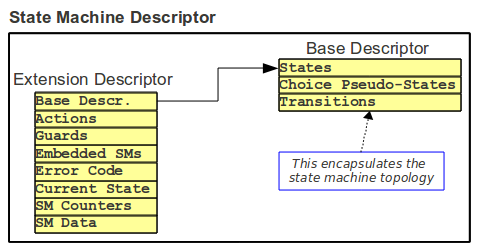
\includegraphics[scale=0.6,keepaspectratio=true]{../images/SMD.png}
 % SMD.png: 474x227 pixel, 72dpi, 16.72x8.01 cm, bb=0 0 474 227
 \caption{Internal Structure of a State Machine Descriptor}
 \label{fig:SMD}
\end{figure}

\subsection{State Machine Module}
The implementation of the state machine concept is split into several files which together
make up the State Machine Module (see Table \ref{tab:swpkg}). The files in the state machine module are listed 
in Table \ref{tab:smModules}.

\begin{longtable}{|p{2.7cm}|p{8.5cm}|}
\caption{Files in State Machine Module} \label{tab:smModules}\\
\hline
\rowcolor{gray}
\textbf{Files} & \textbf{Description} \\
\hline\hline
\texttt{FwSmCore.h}, \texttt{FwSmCore.c}, \texttt{FwSmPrivate.h} & Provide an interface to start and stop a state 
machine and to send a transition command to it. \\
\hline
\texttt{FwSmDCreate.h}, \texttt{FwSmDCreate.c} & Provide an interface to create a new SMD. This interface is 
simple to use but relies on dynamic memory allocation. Applications which wish to avoid dynamic memory 
allocation can use the alternative services of \texttt{FwSmSCreate.h}. \\ 
\hline
\texttt{FwSmSCreate.h}, \texttt{FwSmSCreate.c} & Provide macros to instantiate a new SMD (without using dynamic 
memory allocation) and functions to initialize it. The services in this file are alternative to those of \texttt{FwSmDCreate.h}. \\ 
\hline
\texttt{FwSmConfig.h}, \texttt{FwSmConfig.c}  & Provide an interface to configure a newly created SMD by defining 
its states and transitions. \\
\hline
\texttt{FwSmAux.h}, \texttt{FwSmAux.c} & Provides an interface to auxiliary services which are useful during 
the application development phase. \\
\hline
\end{longtable}

All applications using the C1 Implementation need the \texttt{Core} files. The \texttt{FwSmPrivate.h} header 
file defines the internal structure of an SMD. In most cases, applications can ignore this header file 
and only interact with state machines through the high-level functions declared in the other header files.

\newpage

The \texttt{DCreate} and \texttt{SCreate} files are normally alternative to each other (but deployment of 
both in the same application is possible). Applications which are severely constrained in memory can instantiate 
and configure the SMDs of their state machines by directly manipulating their internal fields. This requires a 
detailed understanding of the internal structure of the SMD but allows an application to dispense with both 
the \texttt{DCreate} and \texttt{SCreate} files and with the \texttt{Config} files. An example of direct instantiation 
and configuration of an SMD is provided in function \texttt{FwSmMakeTestSM5Dir} in the Test Suite. 

 

The \texttt{Aux} files are not intended for inclusion in a final application.

\subsection{State Machine Actions and Guards}
The state machine actions and guards are defined as function pointers of type, respectively, \texttt{FwSmAction\_t} 
and \texttt{FwSmGuard\_t}. Applications must provide functions of these two types to implement the actions and 
guards of their state machines. Both the guard and the action functions are called with the SMD as an argument.

 

Note that, if a state machine uses the same action or the same guard more than once, the associated function 
pointer is only stored once in the SMD. 

\subsection{State Machine Data}\label{sec:smData}
The SMD includes a field holding a pointer to the \emph{state machine data}. The state machine data are data 
which are manipulated by the state machine actions and guards. The exact type of the state machine data is 
defined by applications for each state machine. In most cases, it will take the form a \texttt{struct} whose 
fields represents the inputs and outputs for the state machine actions and guards. The SMD treats the pointer 
to the state machine data as a pointer to \texttt{void}. Functions \texttt{FwSmSetData} and \texttt{FwSmGetData} 
allow this pointer to be set in and to be retrived from an SMD.

 

The FW Profile allows transition commands to carry parameters and to return values. The parameters represent 
the parameters passed to the actions and guards triggered by the transition command and the return values represent the 
values returned by these actions. In the C1 Implementation a transition command is represented by an integer 
identifier and does not directly carry parameters or generate return values. However, the \emph{state machine data} 
can be used as an equivalent mechanism through which a caller of a transition command can exchange data with the 
actions and guards of a state machine.

\subsection{Error Checking}\label{sec:smErrorChecking}
The state machine functions perform a limited amount of error checking. Configuration functions (namely functions 
in module \texttt{FwSmConfig.h}) perform consistency checks on the configuration parameters specified by the user. 
Details can be found in the doxygen description of the configuration functions. 

The functions which trigger a transition in a state machine (namely \texttt{FwSmStart}, \texttt{FwSmMakeTrans}, 
and \texttt{FwSmExecute}) flag the following situations as errors (both of these situations are forbidden by the 
FW Profile):

\begin{fw_itemize}
\item A transition encounters a choice pseudo-state whose out-going transitions all have a false guard
\item A transition is encountered which has a choice pseudo-state as both source and destination
\end{fw_itemize}

Errors are reported through the \emph{error code} field in the SMD which stores the identifier of the last 
error encountered by the implementation. The value of the error code can be read with the \texttt{FwSmGetErrCode} 
function. Nominally, the error code should be equal to \texttt{smSuccess}. If this is not the case, the behaviour 
of the state machine is undefined.

The error codes are listed as enumerated values in file \texttt{FwSmConstants.h}.

\subsection{Else Guards}
An "\emph{Else}" guard is a guard in a transition out of a choice pseudo-state which is true when the guards of 
all other out-going transitions from the same choice pseudo-state are false. "Else" guards are not directly 
supported but their effect can be achieved as follows. The out-going transitions from a choice pseudo-state 
are evaluated in the order in which they were added to the state machine when the state machine was configured. 
If the last transition to be added 
to a choice pseudo-state is given a guard which always returns true, then this transition will behave like 
a transition with an "\emph{Else}" guard.


\subsection{Compliance with UML State Machine Model}
The definition of the state machine concept in UML is complex, often unclear, and sometimes ambiguous. 
The C1 Implementation adopts the state machine model of the FW Profile ~\cite{ref:fwprofile}. 
This is a subset of the UML model which is clearly and unambiguously defined. 

%===============================================================================


\section{Procedure Representation}
This section describes how the procedure concept is implemented in the C1 Implementation. 
This section gives an overview description only. Detailed information is found in the 
Doxygen documentation. The procedure concept is described in appendix \ref{sec:prModel}.

\subsection{Procedure Descriptor}\label{sec:prDesc}
The C1 Implementation represents a procedure through a \emph{procedure descriptor} (PRD). 
A PRD is a data structure which holds all the information required to describe a procedure. 
Users only manipulate pointers to PRDs. These are defined as instances of type \texttt{FwPrDesc\_t}. The internal structure of a PRD is described 
in header file \texttt{FwPrPrivate.h} and is represented in informal notation in Figure \ref{fig:PRD}. 

\begin{figure}[ht]
 \centering
 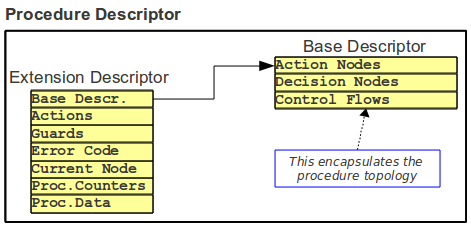
\includegraphics[scale=0.6,keepaspectratio=true]{../images/PRD.png}
 % PRD.png: 474x227 pixel, 72dpi, 16.72x8.01 cm, bb=0 0 474 227
 \caption{Internal Structure of a Procedure Descriptor}
 \label{fig:PRD}
\end{figure}

As shown in the figure, a PRD is internally split into two parts: the \emph{base descriptor} 
and the \emph{extension descriptor}. The base descriptor holds the information which defines 
the topology of the procedure, namely:

\begin{fw_itemize}
\item The list of action nodes in the procedure
\item The list of decision nodes in the procedure
\item The list of control flows in the procedure
\end{fw_itemize}

The extension descriptor holds the information which may be overridden when the procedure 
is extended. This consists of:

\begin{fw_itemize}
\item The list of actions used in the procedure 
\item The list of control flow guards used in the procedure
\item The pointer to the procedure data (the data upon which the procedure actions 
and guards operate, see Section \ref{sec:prData})
\item The current node of the procedure
\item The error code for the procedure (see Section \ref{sec:prErrorChecking})
\item The procedure counters 
\end{fw_itemize}

Applications manipulate a procedure by passing its PRD to the functions defined by 
the C1 Implementation. Thus, for instance, an application executes a procedure through 
the following function call: \texttt{FwPrExecute(prDesc)}. Here, \texttt{prDesc} is the pointer to the PRD of the procedure to be executed. 

In general, applications never need to directly access the internal fields of a PRD. 
They therefore do not need to be concerned with the internal structure of a PRD. Familiarity with the internal PRD structure only becomes important when, for memory or CPU efficiency reasons, users wish to by-pass some of the functions provided by the C1 Implementation and need to directly manipulate the PRD. This is discussed further in section \ref{sec:prUsage}.

\subsection{Procedure Module}
The implementation of the procedure concept is split into several files which together make up the  
Procedure Module (see Table \ref{tab:swpkg}). The files in the state machine module are listed 
in Table \ref{tab:prModule}.

All applications using the C1 Implementation need the \texttt{Core} module. The \texttt{FwPrPrivate.h} header 
file defines the internal structure of a PRD. In most cases, applications can ignore this header file 
and only interact with procedures through the high-level functions declared in the other header files.

The \texttt{DCreate} and \texttt{SCreate} modules are normally alternative to each other (but deployment of 
both in the same application is possible). Applications which are severely constrained in memory can instantiate 
and configure the PRDs of their procedures by directly manipulating their internal fields. This requires a 
detailed understanding of the internal structure of the PRD but allows an application to dispense with both 
the \texttt{DCreate}/\texttt{SCreate} modules and with the \texttt{Config} module. An example of direct instantiation 
and configuration of a PRD is provided in function \texttt{FwPrMakeTestPR2Dir} in the Test Suite. 

\begin{longtable}{|p{2.5cm}|p{8.7cm}|}
\caption{Files in Procedure Module} \label{tab:prModule} \\
\hline
\rowcolor{gray}
\textbf{Files} & \textbf{Description} \\
\hline\hline
\texttt{FwPrCore.h}, \texttt{FwPrCore.c}, \texttt{FwPrPrivate.h} & Provides an interface to start and stop a procedure and 
to send a transition command to it.\\
\hline
\texttt{FwPrDCreate.h}, \texttt{FwPrDCreate.c} & Provides an interface to create a new PRD. This interface is simple to use 
but relies on dynamic memory allocation. Applications which wish to avoid dynamic memory allocation can use the alternative services of \texttt{FwPrSCreate.h}. \\ 
\hline
\texttt{FwPrSCreate.h}, \texttt{FwPrSCreate.c} & Provides macros to instantiate a new PRD (without using dynamic memory allocation) 
and functions to initialize it. This interface is alternative to that of \texttt{FwPrDCreate.h}. \\ 
\hline
\texttt{FwPrConfig.h}, \texttt{FwPrConfig.c}  & Provides an interface to configure a newly created PRD by defining its nodes and control flows. \\
\hline
\end{longtable}

\subsection{Procedure Actions and Guards}
The procedure actions and guards are defined as function pointers of type, respectively, \texttt{FwPrAction\_t} 
and \texttt{FwPrGuard\_t}. Applications must provide functions of these two types to implement the actions and 
guards of their procedures. Both the guard and the action functions are called with the PRD as an argument.

Note that, if a procedure uses the same action or the same guard more than once, the associated function 
pointer is only stored once in the PRD. 

\subsection{Procedure Data}\label{sec:prData}
The PRD includes a field holding a pointer to the \emph{procedure data}. The procedure data are data 
which are manipulated by the procedure actions and guards. The exact type of the procedure data is 
defined by applications for each procedure. In most cases, it will take the form a \texttt{struct} whose 
fields represents the inputs and outputs for the procedure actions and guards. The PRD treats the pointer 
to the procedure data as a pointer to \texttt{void}. Functions \texttt{FwPrSetData} and \texttt{FwPrGetData} 
allow this pointer to be set in and to be retrived from a PRD.

The FW Profile allows execution commands to carry parameters and to return values. The parameters represent 
the parameters passed to the actions and guards triggered by the execution command and the return values represent the 
values returned by the actions. In the C1 Implementation, the execute command (function \texttt{FwPrExecute} 
does not directly carry parameters or generate return values. However, the \emph{procedure data} 
can be used as an equivalent mechanism through which the entity which executes a procedure can exchange data with the 
actions and guards of a procedure.

\subsection{Error Checking}\label{sec:prErrorChecking}
The procedure functions perform a limited amount of error checking. Configuration functions (namely functions 
in module \texttt{FwPrConfig.h}) perform consistency checks on the configuration parameters specified by the user. 
Details can be found in the doxygen description of the configuration functions. 

The \texttt{FwPrExecute} function which executes a procedure flags the following situation as an error:
a decision node is encountered whose out-going control flows all have a false guard.
Note that this situation is explicitly forbidden by the FW Profile.

Errors are reported through the \emph{error code} field in the PRD which stores the identifier of the last 
error encountered by the implementation. The value of the error code can be read with the \texttt{FwPrGetErrCode} 
function. Nominally, the error code should be equal to \texttt{prSuccess}. If this is not the case, the behaviour 
of the procedure is undefined.

The error codes are listed as enumerated values in file \texttt{FwPrConstants.h}.

\subsection{Else Guards}
An "\emph{Else}" guard is a guard in a control fllow out of a decision node which is true when the guards of 
all other out-going control flows from the same decision node are false. "Else" guards are not directly 
supported but their effect can be achieved as follows. The out-going control flows from a decision node
are evaluated in the order in which they were added to the procedure when the procedure was configured. 
If the last control flow to be added 
to a decision node is given a guard which always returns true, then this transition will behave like 
a transition with an "\emph{Else}" guard.

\subsection{Compliance with UML Activity Diagram Model}
The definition of the procedure concept in UML is complex, often unclear, and sometimes ambiguous. 
The C1 Implementation adopts the procedure model of the FW Profile ~\cite{ref:fwprofile}. 
This is a subset of the UML model which is clearly and unambiguously defined. 

%===============================================================================
\section{RT Container Representation}
This section describes how the RT Container concept is implemented in the C1 Implementation. This section gives an overview description only. Detailed information is found in the Doxygen documentation. The RT Container concept is described in appendix \ref{sec:rtContainerModel}.

\subsection{RT Container Descriptor}\label{sec:rtDesc}
The C1 Implementation represents a RT Container through a \emph{RT Container Descriptor} (RTD). An RTD is a data structure which holds all the information required to describe a RT Container and its current state. It is defined as an instance of type: \texttt{struct FwCrDesc}.

Users normally only manipulate pointers to RTDs. The C1 Implementation accordingly defines type \texttt{FwRtDesc\_t} to represent a pointer to an RTD.

Applications manipulate a RT Container by passing its RTD to the functions defined by 
the C1 Implementation. Thus, for instance, an application notifies a RT Container through 
the following function call: \texttt{FwRtNotify(rtDesc)}. Here, \texttt{rtDesc} is the pointer to the RTD of the container to be notified (i.e. it is a variable of type \texttt{FwRtDesc\_t}). 

A RT Container consists of one thread (the \emph{Activation Thread}) and two procedures (the \emph{Activation Procedure} and the \emph{Notification Procedure}). Within the RTD, the Activation Thread is implemented by a POSIX thread. Notification of this thread requires the use a POSIX mutex and a POSIX conditional variable. Both the mutex and the conditional variable are included in the RTD. 

The Activation Procedure and Notification Procedure are represented in the RTD through the pointers to the functions implementing the procedures' actions.

Users may want to exchange data with the container procedures. For this purpose, the RTD includes a field holding a pointer to generic \emph{container data}.

The thread and procedure information are static data which are set when the RT Container is configured and which remain constant afterwards. Additionally, the RTD also holds dynamic data which are updated during the life of the container to reflect the way it is used. The dynamic data consists of: the container state, the value of its notification counter, and the value of its error code.

Thus, in summary, the RTD holds the following data:

\begin{fw_itemize}
\item A POSIX Thread to implement the Activation Thread (see section \ref{sec:activThread})
\item A POSIX Mutex and Condition Variable to support implementation of the notification mechanism for the Activation Thread (see section \ref{sec:notifMechanism})
\item A set of function pointers implementing the actions of the Activation Procedure and of the Notification Procedure (see section \ref{sec:contProc})
\item The container data (see section \ref{sec:contData})
\item The current state of the container (see section \ref{sec:contState})
\item The notification counter (see section \ref{sec:notifMechanism})
\item The error code for the container (see section \ref{sec:rtErrChecking})
\end{fw_itemize} 

The full definition of the RTD can be found in \texttt{FwRtConstants.h}.

\subsection{The Activation Thread}\label{sec:activThread}
The Activation Thread is implemented as a POSIX thread. The thread is completely encapsulated within the RT Container and users of the container do not normally need to interact with it.

The Activation Thread is created and released when the RT Container is started. By default, the thread is created with default values for all its attributes. If non-default values for the thread attributes are desired, the user can use function \texttt{FwRtSetPosixAttr} to load a POSIX thread attribute object with the desired attribute values. 

\subsection{RT Container Procedures}\label{sec:contProc}
A RT Container implements the Activation Procedure and the Notification Procedure. Although these procedures are defined as standard FW Profile procedures, they are implemented within a RT Container without using the Procedure Module of the C1 Implementation. This is done in order to avoid a coupling between the RT Container Module and the Procedure Module of the C1 Implementation. 

The procedure logic shown in figure \ref{fig:RTContainerProcedures} is therefore directly coded into the RT Container. This logic is parameterized with the functions which implement the adaptation points of the two procedures. These functions must be defined by the user when the container is configured.

The procedure functions are loaded into the container as function pointers which must conform to the \texttt{FwRtAction\_t} stereotype. Functions which conform to this stereotype take the container data (see section \ref{sec:contData}) as a parameter and return an integer outcome. The outcome only has a meaning for functions which implement decision points for the procedures namely:

\begin{fw_itemize}
\item \textit{Implement Notification Logic} which determines whether a notification is skipped (return value is 0) or is forwarded (return value is 1)
\item \textit{Implement Activation Logic} which determines whether, in response to a notification, the container's functional behaviour is skipped (return value is 0) or is executed (return value is 1)
\item \textit{Execute Functional Behaviour} which determines whether the container's functional behaviour has terminated (return value is 1) or not (return value is 0)
\end{fw_itemize}

In all other cases, the outcome of the procedure function is a dummy value.

For all procedure functions, default implementations are provided which do nothing and return 1. Thus, users only need to explicitly define a procedure function when its behaviour differs from this default.

The procedure functions may only be defined at configuration time using dedicated setter functions provided by \texttt{FwRtConfig.h}. If these functions are called at other times, they will cause the container to be placed in an error state.

\subsection{Notification Mechanism}\label{sec:notifMechanism}
Users of a RT Container send a notification to the thread encapsulated in the container by calling \texttt{FwRtNotify}. A call to this function triggers the execution of the Notification Procedure. If the notification requests is accepted by the Notification Procedure (this determined by the Implement Notification Logic action in the procedure), the value of the notification counter (variable \texttt{notifCounter} in the RTD) is incremented. The Activation Thread is released whenever the notification counter has a value greater than zero. Every release of the Activation Thread causes the counter to be decremented by 1 (see logic in section \ref{sec:rtContainersBehaviour}). 

Notification requests are therefore buffered by a RT Container. Since variable \texttt{notifCounter} is of type \texttt{FwRtCounterU2\_t}, buffering will be performed up to the point where this type overflows. 

The value of the Notification Counter (which is accessible through function \texttt{FwRtGetNotifCounter}) can also be used to detect overrun situations. An overrun occurs when the (n+1)-th notification is received before the Activation Procedure has completed processing of the n-th notification. This situation has arisen if, when the Activation Procedure is executed, it finds that the Notification Counter has a value greater than zero. 

It is not possible to directly attach data to a notification request. Users can pass data to the notified thread through the "container data" described in section \ref{sec:contData} but these data are not specific to a particular notification request. If a user needs to attach data to a notification request, it must implement a buffer within the container data structure and must implement the buffering logic in the "Implement Notification Logic" function (see figure \ref{fig:RTContainerProcedures}).

\subsection{RT Container State}\label{sec:contState}
The RT Container concept of appendix \ref{sec:rtContainerModel} recognizes two states for a RT Container: STOPPED and STARTED. The RT Container of the C1 Implementation has an expanded set of states which are shown in an informal notation in figure \ref{fig:RTContainerStates}. The nominal states are:

\begin{fw_enumerate}
\item \texttt{rtContUninitialized}: this is the state of the container when it is being configured, i.e. before it is initialized for the first time with function \texttt{FwRtInit} or after it has been shut down with function \texttt{FwRtShutdown}.
\item \texttt{rtContStopped}: this corresponds to state STOPPED as defined by the FW Profile. In the absence of errors, this state is entered when the container has completed its configuration and after it has been stopped with function \texttt{FwRtStop}.
\item \texttt{rtContStarted}: this corresponds to state STARTED as defined by the FW Profile. In the absence of errors, this is the state of the container after it has been successfully started with function \texttt{FwRtStart}  and until it is stopped with function \texttt{FwRtStop}.
\end{fw_enumerate}

Additionally, a number of error states are present. The \texttt{rtConfigErr} state is entered when a configuration function is called during normal operation (i.e. after the container has been initialized with function \texttt{FwRtInit} and before it has been shut down with function \texttt{FwRtShutdown}). An error state is also entered if a POSIX system call fails. For each kind of POSIX system call, an error state is defined. Once the container has entered an error state its behaviour is undefined. For this reason, no out-going transitions from the error states are shown in figure \ref{fig:RTContainerStates}.

The range of values of the container state is defined in type \texttt{FwRtState\_t}. The value of the container state can be read through function \texttt{FwRtGetContState}.
 
\begin{figure}[ht]
 \centering
 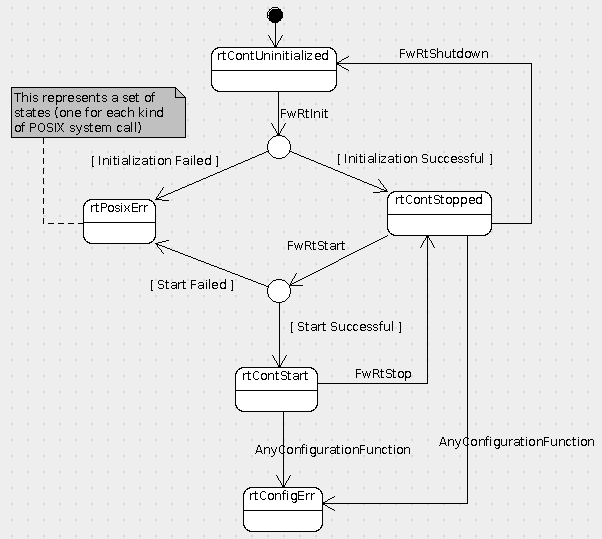
\includegraphics[scale=0.43,keepaspectratio=true]{../images/RTContainerStates.png}
 % PRD.png: 474x227 pixel, 72dpi, 16.72x8.01 cm, bb=0 0 474 227
 \caption{RT Container States}
 \label{fig:RTContainerStates}
\end{figure}

\subsection{Container Data}\label{sec:contData}
The RTD includes a field holding a pointer to the \emph{container data}. The container data are data which are manipulated by the functions in the container procedures. The exact type of the container data is defined by applications for each container. In most cases, it will take the form a \texttt{struct} whose fields represent the inputs and outputs for the procedure functions. The RTD treats the pointer to the container data as a pointer to \texttt{void}. Functions \texttt{FwRtSetData} and \texttt{FwRtGetData} 
allow this pointer to be set in, and to be retrieved from, an RTD.

The container data may also be used as a means to attach data to a notification request (see discussion in section \ref{sec:notifMechanism}).

Note that some of the procedure functions may be called by (at least) two different threads: one or more external threads which notify the container by calling \texttt{FwRtNotify} and the Activation Thread which is internal to the container. If the container data are used to exchange data between these two kinds of procedure functions, then the user must implement protection mechanisms to ensure that these shared data are accessed in mutual exclusion.

\subsection{Error Checking}\label{sec:rtErrChecking}
Two forms of error checks are performed by the RT Container functions:
\begin{fw_enumerate}
\item It is checked that POSIX system calls are successful. A POSIX system call fails if it returns an error code. In that case, the error code is stored in the \texttt{errCode} field of the RTD and the state of the RT Container is set to an error state which depends on the system call which reported the error (e.g. if a call to \texttt{pthread\_mutex\_lock} has failed, the container state is set to \texttt{rtMutexLockErr}).
\item It is checked that configuration functions are only called when the container is being configured (i.e. when it is in state \texttt{rtContUninitialized}). If a configuration function is called during normal operation, the state of the RT Container is set to the error state \texttt{rtConfigErr}.
\end{fw_enumerate} 

If the RT Container is in an error state, its behaviour is undefined. The error states and the error codes are listed as enumerated values in \texttt{FwRtConstants.h}.

%===============================================================================
\section{State Machine Usage}\label{sec:smUsage} 

The basic mode of use of a state machine in the C1 Implementation is as follows:

\begin{fw_itemize}
\item The state machine descriptor (SMD) is created
\item The state machine descriptor is configured
\item The state machine is sent transition commands
\end{fw_itemize}

Examples of creation and configuration of a state machine can be found in the \texttt{FwSmMake*} functions of 
the \texttt{FwSmMakeTest.h} module in the Test Suite. Examples of state machine commanding can be found in the 
\texttt{FwSmTestCases.h} module in the Test Suite and in the Demo Application.

The pseudo-code examples in this section refer to the test state machine SM5 which is shown in Figure \ref{fig:SM5}. 
This test state machine is built by function \texttt{FwSmMakeTestSM5} in the Test 
Suite and it is used in a number of test cases in the test suite.

\begin{figure}[ht]
 \centering
 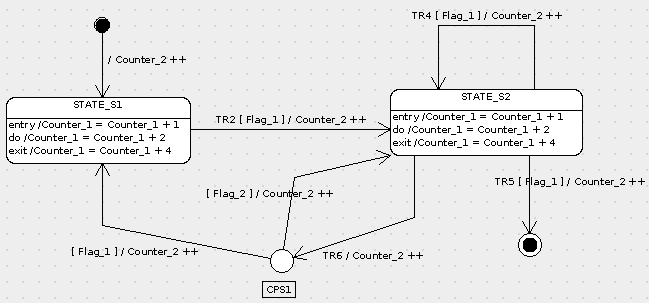
\includegraphics[scale=0.52,keepaspectratio=true]{../images/SM5.png}
 % SMD.png: 474x227 pixel, 72dpi, 16.72x8.01 cm, bb=0 0 474 227
 \caption{Test State Machine SM5}
 \label{fig:SM5}
\end{figure}

\newpage

\subsection{State Machine Descriptor Creation} 
In the state machine creation process, a state machine descriptor together with all its internal data 
structures is instantiated and initialized.

A state machine descriptor can be created in one of three alternative ways as described in Table \ref{tab:smCreation}. 
The last column in the table gives a pointer to one or more functions in the Test Suite where each creation 
method is demonstrated.

\begin{longtable}{|p{1.5cm}|p{6cm}|p{3cm}|}
\caption{Methods to Create a State Machine} \label{tab:smCreation}\\
\hline
\rowcolor{gray}
\textbf{Method} & \textbf{Description} & \textbf{SM Example}\\
\hline\hline
\emph{Dynamic Creation}  & Creation is done through the \texttt{FwSmDCreate} function. The caller specifies 
the size of the state machine and the function allocates the memory for the SMD and its internal data 
structures and returns a pointer to the SMD. This creation interface is simple but relies on dynamic memory 
allocation (malloc). Release of the memory allocated at creation can be done with functions \texttt{FwSmRelease} 
and \texttt{FwSmReleaseRec}. & \texttt{MakeTestSM1}, \texttt{MakeTestSM5} \\
\hline
\emph{Static Creation} & Creation is done in two steps. First, the SMD and its internal data structures are 
instantiated using macro \texttt{FW\_SM\_INST} (if the state machine has choice pseudo-states) or macro
\texttt{FW\_SM\_INST\_NOCPS} (if the state machine has no choice pseudo-states),
and then the SMD and its internal data structures are initialized 
using the \texttt{FwSmInit} function. No dynamic memory allocation is used. & \texttt{MakeTestSM1Static}, \texttt{MakeTestSM5Static}\\
\hline
\emph{Direct Creation} & The application directly instantiates the internal data structures of the state machine 
descriptor. Memory footprint is reduced because neither the \texttt{FwSmDCreate} function nor the \texttt{FwSmInit} 
is needed but users must understand the internal structure of an SMD (this is defined in header 
file \texttt{FwSmPrivate.h}). & \texttt{MakeTestSM5Dir} \\
\hline
\end{longtable}

\newpage

The listings below illustrate the three ways to create an SMD for the case of the test state machine SM5 
(see Figure \ref{fig:SM5}). The characteristics of the state machine are: 2 states, 1 choice pseudo-state, 
7 transitions, 4 actions and 2 guards. With reference to the number of actions and of guards, it is recalled 
that actions which appear more than once are counted only once (in state machine SM5, the state actions appear 
twice because the two states have the same actions and the transition action appears seven times because all 
transitions have the same transition action). Similarly, guards which appear more than once are counted only 
once (in state machine SM5, the guard \texttt{Flag\_1} occurs four times and the guard \texttt{Flag\_2} occurs once).

Note that, in listing \ref{code:dynamicCreationTestSM5} (dynamic creation case), the variable \texttt{smDesc} holds a pointer to the SMD 
whereas in listings \ref{code:staticCreationTestSM5} and \ref{code:directCreationTestSM5} 
(static and direct creation), it holds the SMD itself. Most users should 
use either the approach of listing \ref{code:dynamicCreationTestSM5} or that of listing \ref{code:staticCreationTestSM5}. 
The approach of listing \ref{code:directCreationTestSM5} requires a detailed 
understanding of the internal organization of an SMD and should only be used in applications where memory 
requirements are so tight that it is desirable to drop the SMD creation functions provided by the C1 Implementation.

\lstset{caption={Dynamic Creation of Test State Machine SM5},label=code:dynamicCreationTestSM5}
\begin{lstlisting}
/* Create and initialize the state machine descriptor */
FwSmDesc_t smDesc = FwSmCreate(2, 1, 7, 4, 2);
\end{lstlisting}

\lstset{caption={Static Creation of Test State Machine SM5},label=code:staticCreationTestSM5}
\begin{lstlisting}
/* Instantiate data structures for state machine descriptor */
FW_SM_INST(smDesc, 2, 1, 7, 4, 2)

/* Initialize data structures for state machine descriptor */
FwSmInit(&smDesc);
\end{lstlisting}

\lstset{caption={Direct Creation of Test State Machine SM5},label=code:directCreationTestSM5}
\begin{lstlisting}
/* Instantiate data structures for state machine descriptor */
static SmTrans_t trans[7];
static FwSmAction_t actions[5];
static FwSmGuard_t guards[3];
static SmPState_t pStates[2];
static SmCState_t cStates[1];
static FwSmDesc_t esmDesc[2];
static struct FwSmDesc smDesc;
static SmBaseDesc_t smBase;

/* Initialize state machine descriptor */
smBase.pStates = pStates;
smBase.cStates = cStates;
smBase.trans = trans;
smBase.nOfPStates = 2;
smBase.nOfCStates = 1;
smBase.nOfTrans = 7;
smDesc.smBase = &smBase;
smDesc.transCnt = 0;
smDesc.curState = 0;
smDesc.smData = NULL;
smDesc.nOfActions = 5;
smDesc.nOfGuards = 3;
smDesc.smActions = actions;
smDesc.smGuards = guards;
smDesc.esmDesc = esmDesc;
smDesc.errCode = success;
smDesc.smData = NULL;
\end{lstlisting}

\subsection{State Machine Descriptor Configuration}\label{sec:smConfig}
After being created, an SMD is initialized but is not yet configured. Configuration is done using the functions defined 
in header file \texttt{FwSmConfig.h}. Configuration is done in steps as follows:

\begin{fw_enumerate}
\item The states of the state machine are defined with the \texttt{FwSmAddState} function.  
\item The choice pseudo-states of the state machine are defined with \\ the \texttt{FwSmAddChoicePseudoState} function.
\item The transitions of the state machines are defined with the \texttt{FwSmAddTrans*} functions (there are several 
of these functions, one for each type of transition source and destination).
\item The pointer to the state machine data in the state machine descriptor is set with the \texttt{FwSmSetData} function.
\item The consistency and completeness of the state machine configuration may be verified with function \texttt{FwSmCheck} or \texttt{FwSmCheckRec}. 
\item The configuration of a state machine can be printed with function \\ \texttt{FwSmPrintConfig}.
\end{fw_enumerate}

The only constraint on the order in which these steps are performed is that a transition from a state or 
choice pseudo-state can only be defined after the source state or choice pseudo-state has been defined. 

Configuration of a state machine can only be done once: a state machine which has already been configured 
cannot be configured again.

The pseudo-code in listing \ref{code:configTestSM5} shows configuration steps 1 to 3 for the case of the test state machine SM5 
(see Figure \ref{fig:SM5}). In the pseudo-code, the variables with names like \texttt{incrCnt1By2} ("increment 
counter 1 by 2") are the functions representing the actions in the state machine and the variables with names 
like \texttt{retFlag1} ("return Flag\_1") are the functions representing the guards in the state machine.
The variables CPS1, STATE\_S1 and STATE\_S2 are the identifiers of the choice pseudo-state and of the two
states of the state machine. The variables TR2 to TR6 are the identifiers of the transition commands in the state 
machine.

Note that the identifiers of choice pseudo-states and states must be integers in the range 1 to n where n is,
respectively, the number of choice pseudo-states or the number of states in the state machine. 
The identifiers of the transition commands are non-negative integers but they are not constrained to
be sequential.

Users who are severely constrained in memory can avoid linking the configuration functions by directly 
configuring an SMD and its internal data structures. This, however, requires an understanding of the internal 
structure of an SMD (this is defined in header file \texttt{FwSmPrivate.h}). An example of direct SMD 
configuration can be found in function \texttt{FwSmMakeTestSM5Dir} in the Test Suite. The memory saving of 
taking this approach is about 2 kBytes (this is the memory footprint of the \texttt{FwSmConfig.h} module, 
see Section \ref{sec:memFootprint}). The pseudo-code of listing \ref{code:directConfigTestSM5}
re-casts the pseudo-code of listing \ref{code:configTestSM5} to perform a direct configuration of test 
state machine SM5 (see Figure \ref{fig:SM5}). 

\lstset{caption={Configuration of Test State Machine SM5},label=code:configTestSM5}
\begin{lstlisting}
/* Configure the states */
FwSmAddState(smDesc, STATE_S1, 1, &incrCnt1By1, &incrCnt1By4, &incrCnt1By2, NULL);
FwSmAddState(smDesc, STATE_S2, 3, &incrCnt1By1, &incrCnt1By4, &incrCnt1By2, NULL);

/* Configure  the choice pseudo-state */
FwSmAddChoicePseudoState(smDesc, CPS1, 2);

/* Configure the state transitions */
FwSmAddTransIpsToSta(smDesc, STATE_S1, &incrCnt2By1);
FwSmAddTransStaToSta(smDesc, TR2, STATE_S1, STATE_S2, &incrCnt2By1, &retFlag1);
FwSmAddTransStaToCps(smDesc, TR6, STATE_S2, CPS1, &incrCnt2By1, NULL);
FwSmAddTransCpsToSta(smDesc, CPS1, STATE_S1, &incrCnt2By1, &retFlag1);
FwSmAddTransCpsToSta(smDesc, CPS1, STATE_S2, &incrCnt2By1, &retFlag2);
FwSmAddTransStaToFps(smDesc, TR5, STATE_S2, &incrCnt2By1, &retFlag1);
FwSmAddTransStaToSta(smDesc, TR4, STATE_S2, STATE_S2, &incrCnt2By1, &retFlag1);
\end{lstlisting}


\lstset{caption={Direct Configuration of Test State Machine SM5},label=code:directConfigTestSM5}
\begin{lstlisting}
/* Configure the array of state machine actions */
actions[0] = &SmDummyAction;
actions[1] = &incrCnt1By1;
actions[2] = &incrCnt1By2;
actions[3] = &incrCnt1By4;
actions[4] = &incrCnt2By1;

/* Configure the array of state machine guards */
guards[0] = &SmDummyGuard;
guards[1] = &retFlag1;
guards[2] = &retFlag2;

/* Configure the array of embedded state machines */
esmDesc[0] = NULL;
esmDesc[1] = NULL;

/* Configure the array of proper states */
pStates[0].outTransIndex = 1;
pStates[0].nOfOutTrans = 1;
pStates[0].iEntryAction = 1;
pStates[0].iDoAction = 2;
pStates[0].iExitAction = 3;

pStates[1].outTransIndex = 2;
pStates[1].nOfOutTrans = 3;
pStates[1].iEntryAction = 1;
pStates[1].iDoAction = 2;
pStates[1].iExitAction = 3;

/* Configure the array of choice pseudo-states */
cStates[0].outTransIndex = 5;
cStates[0].nOfOutTrans = 2;

/* Configure the array of transitions */
trans[0].dest = STATE_S1;
trans[0].id = 0;
trans[0].iTrAction = 4;
trans[0].iTrGuard = 0;

trans[1].dest = STATE_S2;
trans[1].id = TR2;
trans[1].iTrAction = 4;
trans[1].iTrGuard = 1;

trans[2].dest = -CPS1;
trans[2].id = TR6;
trans[2].iTrAction = 4;
trans[2].iTrGuard = 0;

trans[3].dest = 0;
trans[3].id = TR5;
trans[3].iTrAction = 4;
trans[3].iTrGuard = 1;

trans[4].dest = STATE_S2;
trans[4].id = TR4;
trans[4].iTrAction = 4;
trans[4].iTrGuard = 1;

trans[5].dest = STATE_S1;
trans[5].id = -1;
trans[5].iTrAction = 4;
trans[5].iTrGuard = 1;

trans[6].dest = STATE_S2;
trans[6].id = -1;
trans[6].iTrAction = 4;
trans[6].iTrGuard = 2;
\end{lstlisting}

\subsection{State Machine Execution}\label{sec:SmExecution}
A state machine is executed by sending it a command to perform a transition. In accordance with the FW Profile, 
before being executed, a state machine must be started. This is done with the \texttt{FwSmStart} function. Applications 
can check whether a state machine has already been started with function \texttt{FwSmIsStarted}.

After a state machine has been started, it will respond to requests to perform a transition (but note that sending 
such a request to a state machine which has not been started is not an error - the request is simply ignored). 
State transitions are exclusively triggered by \emph{transition commands}. Each state machine reacts to a finite 
number of transition commands. Each transition command has an identifier (a non-negative integer). 

The range of transition command identifiers is defined by a user when a state machine is configured. The identifier 0 
is reserved for the \emph{Execute} transition command. The Execute transition command is a transition command which 
triggers the execution of the do-action of the current state of a state machine. The \texttt{\#define} constant 
\texttt{FW\_TR\_EXECUTE} is provided to represent the identifier of the "Execute" transition.

A transition command is sent to a state machine with function \texttt{FwSmMakeTrans}. As a matter of convenience, 
function \texttt{FwSmExecute} is provided to send the Execute command to a state machine.

A state machine is stopped with function \texttt{FwSmStop}. State machines can be started and stopped as many times 
as desired.

The example in listing \ref{code:cmdSeqTestSM5} shows a short commanding sequence for the SM5 state machine. 
In the pseudo-code, variable 
\texttt{smDesc} holds the pointer to the SMD (i.e. variable \texttt{smDesc} is of type \texttt{FwSmDesc\_t}). 
The state machine is first started. This brings it to state \texttt{S1}. The state machine is then sent transition 
commands TR2 and TR6. The response of the state machine to these commands depends on the values of the flags 
\texttt{Flag\_1} and \texttt{Flag\_2}. If, for instance, \texttt{Flag\_1} is true and \texttt{Flag\_2} is false, 
then the first transition command brings the state machine to \texttt{S2} and the second one brings it back to \texttt{S1}.

\lstset{caption={Commanding Sequence for Test State Machine SM5},label=code:cmdSeqTestSM5}
\begin{lstlisting}
/* Start the state machine */
FwSmStart(smDesc);

/* Send transition command TR2 to the state machine */
FwSmMakeTrans(smDesc, TR2);

/* Send transition command TR6 to the state machine */
FwSmMakeTrans(smDesc, TR6);

/* Stop the state machine */
FwSmStop(smDesc);
\end{lstlisting}

\subsection{State Machine Extension}
The C1 Implementation supports an extension mechanism for state machines which is similar to the inheritance-based 
extension mechanism of object-oriented languages. The extension mechanism is \emph{optional}: there is no requirement 
that all applications using the C1 Implementation also use the extension mechanism.



A state machine (the \emph{base state machine}) can be \emph{extended} to create a new state machine 
(the \emph{derived state machine}). A derived state machine can either be created dynamically with the 
\texttt{FwSmDCreateDer} function or else it can be instantiated statically with macro \texttt{FW\_SM\_INST\_DER} and 
initialized with function \texttt{FwSmInitDer}.



After being created, a derived state machine is a clone of its base. It can then be configured by performing 
one or more of the following operations: 

\begin{fw_itemize}
\item Overriding its actions (through function \texttt{FwSmOverrideAction})
\item Overriding its guards (through function \texttt{FwSmOverrideGuard}) 
\item Embedding new state machines in its states (through function \texttt{FwSmEmbed}).
\end{fw_itemize}

The internal structure of the SMD is designed to minimize the memory requirements of derived state machines
(see Figure \ref{fig:SMD}). An SMD is split into two parts: the Base Descriptor and the Extension 
Descriptor. The Base Descriptor holds the information about the state machine topology (its states, choice 
pseudo-states and their connections) whereas the Extension Descriptor holds the information about the state 
machine actions and guards and its embedded state machines. During the extension process, only the Extension 
Descriptor is duplicated whereas the Base Descriptor is shared between a state machine and its children 
(see Figure \ref{fig:SMDExtension}). This significantly reduces memory occupation in a situation where a 
large number of state machines are derived from the same base state machine. 

\begin{figure}[ht]
 \centering
 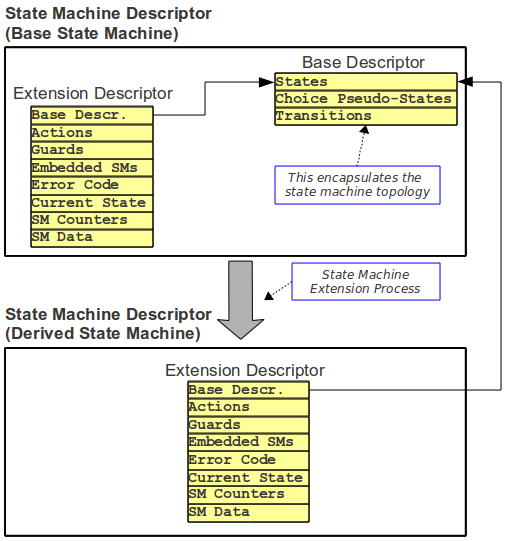
\includegraphics[scale=0.52,keepaspectratio=true]{../images/SMDExtension.png}
 % SMD.png: 474x227 pixel, 72dpi, 16.72x8.01 cm, bb=0 0 474 227
 \caption{Extension Mechanism for State Machine Descriptors}
 \label{fig:SMDExtension}
\end{figure}

The extension mechanism is useful where there is a need to define a large number of state machines which share 
the same topology (same set of states, of choice pseudo-states, and of transitions) but differ either in their 
actions, or in their guards, or in the internal behaviour of their states.

As an example, consider an application which manages a set of external hardware devices all of which are 
characterized by the same basic states (e.g. OFF, STANDBY, OPERATIONAL) and by the same behaviour in states OFF 
and OPERATIONAL, but which have different and device-specific behaviour in state STANDBY. In this case, it is 
convenient to proceed as follows:

\begin{fw_itemize}
\item A base state machine is defined to model the behaviour which is shared by all devices
\item For each device, a state machine is derived which overrides the behaviour in state STANDBY in a manner 
that is specific to each device.
\end{fw_itemize}

The Demo Application offers another example of a situation where the extension mechanism is useful. In this 
application, several Failure Detection (FD) Checks must be implemented for the same Hardware Device. All FD 
Checks share the same basic behaviour: they can be enabled and disabled and, when they are enabled, they can 
either declare the device to be healthy or they can declare it to have failed. The algorithm which is used to 
declare the device healthy or failed is, however, specific to each FD Check. The application is therefore organized 
as follows:

\begin{fw_itemize}
\item A base state machine is defined to model the behaviour which is shared by all FD Checks
\item For each FD Check, a state machine is derived which overrides the algorithm to check the health of the device
\end{fw_itemize}

The pseudo-code in listing \ref{code:dynamicCreationConfigDerSM} offers a concrete example of creation and 
configuration of a derived state machine. 
The state machine of Figure \ref{fig:SM5} acts as \emph{base state machine} and it is extended to create a new state 
machine (the \emph{derived state machine}) as shown in Figure \ref{fig:SMDExtension}. The derived state machine has 
overridden the entry action of the two states and the guard on the transition from the choice pseudo-state to state 
\texttt{S2}. Note that it would not have been possible to override only the entry action of state \texttt{S1}. The entry actions 
of the two states \texttt{S1} and \texttt{S2} have been defined to be identical and are implemented by the same function 
\texttt{incrCnt1By1} (see configuration examples in the previous sections) and can therefore only be overridden together. 

In the example of listing \ref{code:dynamicCreationConfigDerSM}, the descriptor of the derived state machine is created dynamically by 
function \texttt{FwSmCreateDer}. For users who do not wish to rely on dynamic memory allocation, an alternative approach 
is available which is illustrated in listing \ref{code:staticCreationConfigDerSM}. 
Note that in listing \ref{code:dynamicCreationConfigDerSM} the first example variable \texttt{smDescDer} is 
a pointer to the state machine descriptor whereas in listing \ref{code:staticCreationConfigDerSM} it is the state machine descriptor itself.

Use of the derived state machine is done as in the case of non-derived state machines and the examples of section \ref{sec:SmExecution} 
remain therefore applicable.


\lstset{caption={Dynamic Creation and Configuration of Derived State Machine},label=code:dynamicCreationConfigDerSM}
\begin{lstlisting}
/* Create the derived state machine (smDesc is the pointer to the SMD of the base SM) */
FwSmDesc_t smDescDer = FwSmCreateDer(smDesc);

/* Override Action incrCnt1By1 with action incrCnt1By8 */
FwSmOverrideAction(smDescDer, &incrCnt1By1, &incrCnt1By8);

/* Override Guard retFlag1 with gurd retFlag3 */
FwSmOverrideGuard(smDescDer, &retFlag1, &retFlag3);
\end{lstlisting}

\noindent\begin{minipage}{\textwidth}
\lstset{caption={Static Creation and Configuration of Derived State Machine},label=code:staticCreationConfigDerSM}
\begin{lstlisting}
/* Instantiate derived SM with 2 states, 4 actions and 2 guards */
FW_SM_INST_DER(smDescDer, 2, 4, 2)

/* Create the derived state machine (smDesc is the pointer to the SMD of the base SM) */
FwSmInitDer(&smDescDer, smDesc);

/* Override Action incrCnt1By1 with action incrCnt1By8 */
FwSmOverrideAction(&smDescDer, &incrCnt1By1, &incrCnt1By8);

/* Override Guard retFlag1 with guard retFlag3 */
FwSmOverrideGuard(&smDescDer, &retFlag1, &retFlag3);
\end{lstlisting}
\end{minipage}

%===============================================================================
\section{Procedure Usage}\label{sec:prUsage}

The basic mode of use of a procedure in the C1 Implementation is as follows:

\begin{fw_itemize}
\item The procedure descriptor (PRD) is created
\item The procedure descriptor is configured
\item The procedure is executed
\end{fw_itemize}

Examples of creation and configuration of a procedure can be found in the \texttt{FwPrMake*} functions of 
the \texttt{FwPrMakeTest.h} module in the Test Suite. Examples of procedure execution can be found in the 
\texttt{FwPrTestCases.c} module in the Test Suite and in the Demo Application.

The pseudo-code examples in this section refer to the test procedure PR2 which is shown in Figure \ref{fig:PR2}. 
This test procedure is built by function \texttt{FwPrMakeTestPR2} in the Test 
Suite and it is used in a number of test cases in the test suite.

\begin{figure}[ht]
 \centering
 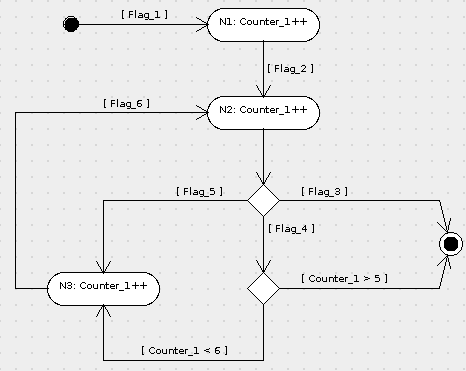
\includegraphics[scale=0.52,keepaspectratio=true]{../images/PR2.png}
 % PRD.png: 474x227 pixel, 72dpi, 16.72x8.01 cm, bb=0 0 474 227
 \caption{Test procedure PR2}
 \label{fig:PR2}
\end{figure}

\newpage

\subsection{Procedure Descriptor Creation} 
In the procedure creation process, a procedure descriptor together with all its internal data 
structures is instantiated and initialized.

A procedure descriptor can be created in one of three alternative ways as described in Table \ref{tab:prCreation}. 
The last column in the table gives a pointer to one or more functions in the Test Suite where each creation 
method is demonstrated.

\begin{longtable}{|p{1.5cm}|p{6cm}|p{3cm}|}
\caption{Methods to Create a Procedure} \label{tab:prCreation}\\
\hline
\rowcolor{gray}
\textbf{Method} & \textbf{Description} & \textbf{Proc. Example}\\
\hline\hline
\emph{Dynamic Creation}  & Creation is done through the \texttt{FwPrDCreate} function. The caller specifies 
the size of the procedure and the function allocates the memory for the PRD and its internal data 
structures and returns a pointer to the PRD. This creation interface is simple but requires dynamic memory 
allocation (\texttt{malloc}). Release of the memory allocated at creation can be done with function \texttt{FwPrRelease}. 
& \texttt{MakeTestPR1}, \texttt{MakeTestPR2} \\
\hline
\emph{Static Creation} & Creation is done in two steps. First, the PRD and its internal data structures are 
instantiated using either macro \texttt{FW\_PR\_INST} (if the procedure has at least one decision node) or
macro \texttt{FW\_PR\_INST\_NODEC} (if the procedure has no decision nodes), and then the PRD and its 
internal data structures are initialized 
using the \texttt{FwPrInit} function. No dynamic memory allocation is used. & \texttt{MakeTestPR1Static}, \texttt{MakeTestPR2Static}\\
\hline
\emph{Direct Creation} & The application directly instantiates the internal data structures of the procedure 
descriptor. Memory footprint is reduced because neither the \texttt{FwPrDCreate} function nor the \texttt{FwPrInit} 
function is needed but users must understand the internal structure of a PRD (this is defined in header 
file \texttt{FwPrPrivate.h}). & \texttt{MakeTestPR2Dir} \\
\hline
\end{longtable}

\newpage

The examples of listing \ref{code:dynamicCreationTestPR2} to \ref{code:directCreationTestPR2} illustrate the 
three ways to create a PRD for the case of the test procedure PR2 
(see Figure \ref{fig:PR2}). The characteristics of the procedure are: 3 action nodes, 2 decision nodes, 
9 control flows, 1 action (used in several actions nodes), and 8 guards. 
With reference to the number of actions and of guards, it is recalled that actions and guards which appear 
more than once  are counted only once 
(in procedure PR2, the action to increment \texttt{Counter\_1} by 1 occurs three times).
Note that, in listing \ref{code:dynamicCreationTestPR2} (dynamic creation case), the variable \texttt{prDesc} 
holds a pointer to the PRD whereas in listings \ref{code:staticCreationTestPR2} and \ref{code:directCreationTestPR2} 
(static and direct creation), it holds the PRD itself.

Most users should use either the approach of listing \ref{code:dynamicCreationTestPR2} or that of llisting
\ref{code:staticCreationTestPR2}. The approach of listing \ref{code:directCreationTestPR2} 
requires a detailed understanding of the internal organization of a PRD and should only be used in 
applications where memory requirements are so tight that it is desirable to drop the PRD creation 
functions provided by the C1 Implementation.

\lstset{caption={Dynamic Creation of Test Procedure PR2},label=code:dynamicCreationTestPR2}
\begin{lstlisting}
/* Create and initialize the procedure descriptor */
FwPrDesc_t prDesc = FwPrCreate(3, 2, 9, 1, 8);
\end{lstlisting}

\lstset{caption={Static Creation of Test Procedure PR2},label=code:staticCreationTestPR2}
\begin{lstlisting}
/* Instantiate data structures for procedure descriptor */
FW_PR_INST(prDesc, 3, 2, 9, 1, 8)

/* Initialize data structures for procedure descriptor */
FwPrInit(&prDesc);
\end{lstlisting}

\lstset{caption={Direct Creation of Test Procedure PR2},label=code:directCreationTestPR2}
\begin{lstlisting}
/* Instantiate data structures for procedure descriptor */
static PrANode_t aNodes[3];	        
static PrDNode_t dNodes[2]; 	        
static PrFlow_t flows[9];	        
static FwPrAction_t actions[1]; 
static FwPrGuard_t guards[9];	
static PrBaseDesc_t prBase;
static struct FwPrDesc prDesc;

/* Initialize procedure descriptor */
prBase.aNodes = aNodes;
prBase.dNodes = dNodes;
prBase.flows = flows;
prBase.nOfANodes = 3;
prBase.nOfDNodes = 2;
prBase.nOfFlows = 9;
prDesc.curNode = 0;
prDesc.errCode = prSuccess;
prDesc.flowCnt = 0;
prDesc.nOfActions = 1;
prDesc.nOfGuards = 9;
prDesc.prActions = actions;
prDesc.prBase = prBase;
prDesc.prData = prData;
prDesc.prGuards = guards;
prDesc.prData = NULL;
\end{lstlisting}

\subsection{Procedure Descriptor Configuration}\label{sec:prConfig}
After being created, a PRD is initialized but is not yet configured. Configuration is done using the functions defined 
in header file \texttt{FwPrConfig.h}. Configuration is done in steps as follows:

\begin{fw_enumerate}
\item The action nodes of the procedure are defined with the \texttt{FwPrAddAction\-Node} function.  
\item The decision nodes of the procedure are defined with the \texttt{FwPrAdd\-Deci\-sion\-Node} function.
\item The control flows of the procedures are defined with the \texttt{FwPrAddFlow*} functions (there are several of these functions, 
one for each type of control flow source and destination).
\item The pointer to the procedure data in the procedure descriptor is set with the \texttt{FwPrSetData} function.
\item The consistency and completeness of the procedure configuration may be verified with function \texttt{FwPrCheck}. 
\end{fw_enumerate}

The only constraint on the order in which these steps are performed is that a control flow 
can only be defined after its source node has been defined. 

Configuration of a procedure can only be done once: a procedure which has already been configured 
cannot be configured again.

Listing \ref{code:configTestPR2} shows configuration steps 1 to 3 for the case of the test procedure PR2 
(see Figure \ref{fig:PR2}). In the pseudo-code, the variable \texttt{incrCnt1By1} ("increment 
counter 1 by 1") is the function representing the actions in the procedure and the variables with names 
like \texttt{retFlag1} ("return Flag\_1")are the functions representing the guards in the procedure.

Users who are severely constrained in memory can avoid linking the configuration functions by directly 
configuring a PRD and its internal data structures. This, however, requires an understanding of the internal 
structure of a PRD (this is defined in header file \texttt{FwPrPrivate.h}). An example of direct PRD 
configuration can be found in function \texttt{FwPrMakeTestPR2Dir} in the Test Suite. The memory saving of 
taking this approach is about 2 kBytes (this is the memory footprint of the \texttt{FwPrConfig.h} module, 
see Section \ref{sec:memFootprint}). 
Listing \ref{code:directConfigTestPR2} re-casts the example of listing \ref{code:configTestPR2}
to perform a direct configuration of test procedure PR2 (see Figure \ref{fig:PR2}). 

\lstset{caption={Configuration of Test Procedure PR2},label=code:configTestPR2}
\begin{lstlisting}
/* Configure the action nodes */
FwPrAddActionNode(prDesc, N1, &incrCnt1By1);
FwPrAddActionNode(prDesc, N2, &incrCnt1By1);
FwPrAddActionNode(prDesc, N3, &incrCnt1By1);

/* Configure  the decision nodes */
FwPrAddDecisionNode(prDesc, D1, 3);
FwPrAddDecisionNode(prDesc, D2, 2);

/* Configure the control flows */
FwPrAddFlowIniToAct(prDesc, N1, &retFlag1);
FwPrAddFlowActToAct(prDesc, N1, N2, &retFlag2);
FwPrAddFlowActToDec(prDesc, N2, D1, NULL);
FwPrAddFlowDecToFin(prDesc, D1, &retFlag3);
FwPrAddFlowDecToDec(prDesc, D1, D2, &retFlag4);
FwPrAddFlowDecToAct(prDesc, D1, N3, &retFlag5);
FwPrAddFlowActToAct(prDesc, N3, N2, &retFlag6);
FwPrAddFlowDecToAct(prDesc, D2, N3, &returnCounter1SmallerThan6);
FwPrAddFlowDecToFin(prDesc, D2, &returnCounter1GreaterThan5);
\end{lstlisting}


\lstset{caption={Direct Configuration of Test Procedure PR2},label=code:directConfigTestPR2}
\begin{lstlisting}
/* Configure the array of procedure actions */
actions[0] = &incrCnt1By1;

/* Configure the array of procedure guards */
guards[0] = &PrDummyGuard;
guards[1] = &retFlag1;
guards[2] = &retFlag2;
guards[3] = &retFlag3;
guards[4] = &retFlag4;
guards[5] = &retFlag5;
guards[6] = &retFlag6;
guards[7] = &returnCounter1GreaterThan5;
guards[8] = &returnCounter1SmallerThan6;

/* Configure the array of action nodes */
aNodes[0].iAction = 0;
aNodes[0].iFlow = 1;
aNodes[1].iAction = 0;
aNodes[1].iFlow = 2;
aNodes[2].iAction = 0;
aNodes[2].iFlow = 3;

/* Configure the array of decision nodes */
dNodes[0].nOfOutTrans = 3;
dNodes[0].outFlowIndex = 4;
dNodes[1].nOfOutTrans = 2;
dNodes[1].outFlowIndex = 7;

/* Configure the array of control flows */
flows[0].dest = 1;
flows[0].iGuard = 1;
flows[1].dest = 2;
flows[1].iGuard = 2;
flows[2].dest = -1;
flows[2].iGuard = 0;
flows[3].dest = 2;
flows[3].iGuard = 6;
flows[4].dest = 3;
flows[4].iGuard = 5;
flows[5].dest = -2;
flows[5].iGuard = 4;
flows[6].dest = 0;
flows[6].iGuard = 3;
flows[7].dest = 3;
flows[7].iGuard = 8;
flows[8].dest = 0;
flows[8].iGuard = 7;
\end{lstlisting}

\subsection{Procedure Execution}\label{sec:PrExecution}
In accordance with the FW Profile, 
before being executed, a procedure must be started. This is done with the \texttt{FwPrStart} function. Applications 
can check whether a procedure has already been started with function \texttt{FwPrIsStarted}.

After a procedure has been started, it will respond to execution requests (but note that sending 
such a request to a procedure which has not been started is not an error - the execution request is simply ignored). 
An execution request is sent to a procedure by means of function \texttt{FwPrExecute}. 

A procedure is stopped with function \texttt{FwPrStop}. Procedures can be started and stopped as many times 
as desired.

Listing \ref{code:cmdSeqTestPR2} shows a short commanding sequence for the PR2 procedure. In the pseudo-code, variable 
\texttt{prDesc} holds the pointer to the PRD (i.e. variable \texttt{prDesc} is of type \texttt{FwPrDesc\_t}). 
The procedure is first started. 
It is then executed twice and it is finally stopped. 
The response of the procedure to these commands depends on the values of the flags \texttt{Flag\_1} and \texttt{Flag\_2}. 
If, for instance, \texttt{Flag\_1} is true and \texttt{Flag\_2} is false, then the first execution command brings 
the procedure to N1 (causing its action to be executed) and the second one has no effect.


\lstset{caption={Commanding Sequence for Test Procedure PR2},label=code:cmdSeqTestPR2}
\begin{lstlisting}
/* Start the procedure */
FwPrStart(prDesc);

/* Send first execution command to the procedure */
FwPrExecute(prDesc);

/* Send second execution command to the procedure */
FwPrExecute(prDesc);

/* Stop the procedure */
FwPrStop(prDesc);
\end{lstlisting}

\subsection{Procedure Extension}
The C1 Implementation supports an extension mechanism for procedures which is similar to the inheritance-based 
extension mechanism of object-oriented languages. The extension mechanism is \emph{optional}: there is no requirement 
that all applications using the C1 Implementation also use the extension mechanism.

A procedure (the \emph{base procedure}) can be \emph{extended} to create a new procedure 
(the \emph{derived procedure}). A derived procedure can either be created dynamically with the 
\texttt{FwPrDCreateDer} function or else it can be instantiated statically with macro \texttt{FW\_PR\_INST\_DER} and 
initialized with function \texttt{FwPrInitDer}.


After being created, a derived procedure is a clone of its base. It can then be configured by performing 
one or more of the following operations: 

\begin{fw_itemize}
\item Overriding its actions (through function \texttt{FwPrOverrideAction})
\item Overriding its guards (through function \texttt{FwPrOverrideGuard}) 
\end{fw_itemize}

The internal structure of the PRD is designed to minimize the memory requirements of derived procedures
(see Figure \ref{fig:PRD}). A PRD is split into two parts: the Base Descriptor and the Extension 
Descriptor. The Base Descriptor holds the information about the procedure topology (its nodes and the control
flows connecting them) whereas the Extension Descriptor holds the information about the procedure 
actions and guards and the procedure state. During the extension process, only the Extension 
Descriptor is duplicated whereas the Base Descriptor is shared between a procedure and its children 
(see Figure \ref{fig:PRDExtension}. This significantly reduces memory occupation in a situation where a 
large number of procedures are derived from the same base procedure. 



\begin{figure}[ht]
 \centering
 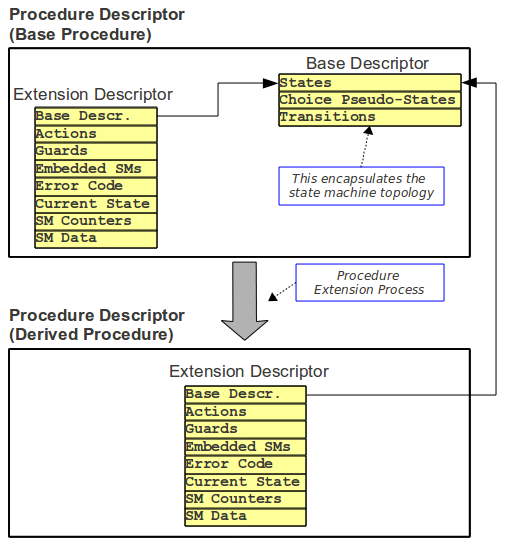
\includegraphics[scale=0.52,keepaspectratio=true]{../images/PRDExtension.png}
 % PRD.png: 474x227 pixel, 72dpi, 16.72x8.01 cm, bb=0 0 474 227
 \caption{Extension Mechanism for Procedure Descriptors}
 \label{fig:PRDExtension}
\end{figure}

The extension mechanism is useful where there is a need to define a large number of procedures which share 
the same topology (same set of action nodes, of decision nodes, and of control flows) but differ either in their 
actions or in their guards.



As an example, consider an application which manages a set of hardware devices all of which must be
initialized by performing a sequence of elementary operations and suppose that all devices share the same
logical sequence of initialization operations (e.g. power-on, switch-on, self-test command, and then, depending
on the outcome of the self-test, either a power-off or a command to enter normal operational state). 
Suppose, however, that the self-tests differ across devices. 
In this case, it is convenient to proceed as follows:

\begin{fw_itemize}
\item A base procedure is defined to model the behaviour which is shared by all devices.
\item For each device, a procedure is derived which overrides the action nodes corresponding to the 
execution of the self-test and the guard which evaluates its outcome.
\end{fw_itemize}

The pseudo-code of listing \ref{code:dynamicCreationConfigDerPR} offers a concrete example of creation and 
configuration of a derived procedure. 
The procedure of Figure \ref{fig:PR2} acts as \emph{base procedure} and it is extended to create a new 
procedure (the \emph{derived procedure}). 
The derived procedure differs from the base procedure in that it has a different action
(\texttt{incrCnt1By8} instead of \texttt{incrCnt1By1}) in its three nodes N1, N2 and N3.
Note that it would not have been possible to override only the action of state N1. 
The actions of the three nodes N1 to N3 have been defined to be identical and are 
implemented by the same function \texttt{incrCnt1By1} (see configuration examples in the previous section) 
and can therefore only be overridden together. 

In listing \ref{code:dynamicCreationConfigDerPR}, the descriptor of the derived procedure is created dynamically by 
function \texttt{FwPrCreateDer}. For users who do not wish to rely on dynamic memory allocation, an alternative approach 
is available which is illustrated in listing \ref{code:staticCreationConfigDerPR}. 
Note that in listing \ref{code:dynamicCreationConfigDerPR} variable \texttt{prDescDer} is 
a pointer to the procedure descriptor whereas in listing \ref{code:staticCreationConfigDerPR} it is the procedure descriptor itself.

Use of the derived procedure is done as in the case of non-derived procedures and the examples of section \ref{sec:PrExecution} 
remain therefore applicable.


\lstset{caption={Dynamic Creation and Configuration of Derived Procedure},label=code:dynamicCreationConfigDerPR}
\begin{lstlisting}
/* Create the derived procedure (psDesc is the pointer to the PRD of the base SM) */
FwPrDesc_t prDescDer = FwPrCreateDer(prDesc);

/* Override Action incrCnt1By1 with action incrCnt1By8 */
FwPrOverrideAction(prDescDer, &incrCnt1By1, &incrCnt1By8);

\end{lstlisting}


\lstset{language=C,caption={Static Creation and Configuration of Derived Procedure},label=code:staticCreationConfigDerPR}
\begin{lstlisting}
/* Instantiate the derived PR with 1 actions and 8 guards */
FW_PR_INST_DER(prDescDer, 1, 8)

/* Initialize the derived procedure (prDesc is the pointer to the PRD of the base SM) */
FwPrInitDer(&prDescDer, prDesc);

/* Override Action incrCnt1By1 with action incrCnt1By8 */
FwPrOverrideAction(&prDescDer, &incrCnt1By1, &incrCnt1By8);
\end{lstlisting}


%===============================================================================
\section{RT Container Usage}\label{sec:rtUsage}

The basic mode of use of a RT Container in the C1 Implementation is as follows:

\begin{fw_itemize}
\item The RT Container Descriptor (RTD) is created
\item The RT Container Descriptor is configured
\item The RT Container is sent notification requests 
\item The RT Container is shut down
\end{fw_itemize}

Examples of creation and configuration of a RT Container can be found in the \texttt{FwRtMake*} functions of the \texttt{FwRtMakeTest.h} module in the Test Suite. Examples of notifications of RT Containers can be found in the \texttt{FwRtTestCases.c} module in the Test Suite.

The pseudo-code examples in this section refer to a simple test container which, every time it receives a notification, writes a message to standard output. The full code for the example is defined in the "RT Container Coding Example 1" (file \texttt{FwProfile\_RtExample1.c} in the delivery file of the C1 Implementation).  

\subsection{RT Container Descriptor Creation}\label{sec:rtCreation}
A RT Container Descriptor (RTD) is a variable of type \texttt{struct FwRtDesc}. A container instance is created as in listing \ref{code:creationRtCont}.
Note that instantiation of the RTD also instantiates the POSIX thread which implements the Activation Thread and the POSIX mutex and POSIX condition variable which support its use. 

\lstset{caption={Creation of a RT Container Instance},label=code:creationRtCont}
\begin{lstlisting}
/* Instantiate a RT Container Descriptor */
struct FwRtDesc rtDesc;
\end{lstlisting}

 
\subsection{RT Container Descriptor Configuration}\label{sec:rtConfiguration}
After being created, an RTD must be configured. Configuration is done using the functions defined in header file \texttt{FwRtConfig.h}. Configuration is done in steps as follows:

\begin{fw_enumerate}
\item The RTD is reset.  
\item The attributes of the POSIX objects encapsulated in the RTD are set.
\item The functions implementing the actions of the container's Activation Procedure and Notification Procedure are set.
\item The container data are set.
\item The RTD is initialized.  
\end{fw_enumerate}

The reset operation must be done first and the initialization operation must be done last. The other three operations may be done in any order. A container may be configured multiple times but configuration may only be done when the container is in state \texttt{rtContUninitialized}, i.e. before it has been initialized or after it has been shut down (see section \ref{sec:contState}). 

The RTD is reset through function \texttt{FwRtReset}. Execution of this function initializes all fields of the RTD to dummy but valid values (the full list of the initialization values can be found in the Doxygen documentation). Thus, after being reset, the RTD is ready to be initialized (but, after being initialized, will not be able to do anything meaningful). Reset of the test container is done at line 17 in listing \ref{code:configRtCont}.

A RT Container uses three POSIX objects: a POSIX thread, a POSIX mutex, and a POSIX condition variable. By default, all three objects are created with the POSIX-defined default values for their attributes. If a user wishes to configure any of these objects with non-default attribute values, he should:

\begin{fw_enumerate}
\item Instantiate an attribute object of the appropriate type (for instance, of type \texttt{pthread\_attr\_t} for the POSIX thread attributes).  
\item Configure the attribute object as desired using the functions defined by POSIX.
\item Load the configured attribute object into the RTD by means of function \texttt{FwRtSetPosixAttr}.
\end{fw_enumerate}

In the test container, default values are used and hence none of the above steps is executed.

By default, the functions implementing the actions of the container's Activation Procedure and Notification Procedure are initialized to dummy functions which do nothing and always return 1. For each such function, the \texttt{FwRtConfig.h} module offers a setter and a getter function which can be used to set and read the corresponding procedure function. Thus, for instance, functions \texttt{FwRtSetInitializeActivPr} and \texttt{FwRtGetInitializeActivPr} can be used to set and get the the function which implements the initialization action for the Activation Procedure.

At a minimum, the user should load a non-trivial Functional Behaviour through function \texttt{FwRtSetExecFuncBehaviour}. The function thus loaded defines the behaviour executed by the Activation Thread when it is notified. In the case of the test container considered in this section, function \texttt{UserFunctionalBehaviour} in listing \ref{code:configRtCont} represents the user-defined functional behaviour which is executed when the container is notified. This behaviour is encapsulated in a function whose pointer is passed to the container through the call to function \texttt{FwRtSetExecFuncBehaviour} in the last line of listing \ref{code:configRtCont}.

Other aspects of a container's behaviour (e.g. the behaviour it should execute when it is initialized or when it is shut down) can be defined in a similar way by first defining a function ecapsulating the desired behaviour and by then loading a pointer to that function into the container using the appropriate setter function (e.g. the initialization function for the Activation Thread is loaded using function \texttt{FwRtSetInitializeActivPr}).

The final step in the configuration process of a RT Container is the definition of the container data (see section \ref{sec:contData}). This is only needed in the case where either data must be passed to the container when it is notified or some of the container functions must exchange data with each other. The container data are loaded into the container using function \texttt{FwRtSetData}. In the case of the test container, no container data are needed and this function is therefore not used.

\lstset{caption={Configuration of a RT Container Instance},label=code:configRtCont}
\begin{lstlisting}
/**
 * Function implementing the user's functional behaviour.
 * In this example, this function prints a message and returns zero.
 * @param rtDesc the RT Container descriptor
 * @return always return zero
 */
FwRtOutcome_t UserFunctionalBehaviour(FwRtDesc_t rtDesc) {
	static int i = 1;
	printf("Activation Thread: Notification %i has been received!\n",i);
	i++;
	return 0;
}

 . . .

/* Reset the RT Container */
FwRtReset(&rtDesc);

/* Attach functional behaviour to RT Container */
FwRtSetExecFuncBehaviour(&rtDesc,&UserFunctionalBehaviour);

/* Initialize the RT Container */
FwRtInit(&rtDesc);
\end{lstlisting}

\subsection{RT Container Descriptor Notification}\label{sec:rtNotification}
In accordance with the FW Profile, before being able to process notification requests, a RT Container must be started. This is done with the \texttt{FwRtStart} function. Applications can check whether a RT Container has already been started with function \texttt{FwRtGetContState} which returns the container's state.

After a RT Container has been started, it will respond to notification requests (but note that sending such a request to a container which has not been started is not an error - it simply means that the notification request is ignored). A notification request is sent to a RT container by means of function \texttt{FwRtNotify}. 

A RT Container is stopped with function \texttt{FwRtStop}. After being stopped, the container terminates the Activation Thread and no longer processes notification requests but it may still hold some system resources. If it is desired to ensure that all such resources are released, the container must be shut down by means of function \texttt{FwRtShutdown}. This function destroys the POSIX objects used by the container and releases any system resources they may have claimed.

After a RT Container has been stopped, it can be re-started. The start-stop cycle can be executed as many times as desired. After it has been shut down, the container must be re-configured anew before it can again be used.

When a RT Container is stopped (or when it terminates autonomously because its functional behaviour has terminated execution), its Activation Thread is terminated. A RT Container should only be shut down or re-started after the Activation Thread has terminated. As a convenience, the RT Container provides function \texttt{FwRtWaitForTermination} to wait until the Activation Thread has terminated. This function is implemented using POSIX's \texttt{pthread\_join} system call.

Listing \ref{code:notifRtCont} shows a sequence of ten notifications separated by waits of 10 milliseconds for the test container. After the notifications have been sent, the container is stopped and (after its Activation Thread has terminated execution), it is shutdown.

\lstset{caption={Notification of a RT Container Instance},label=code:notifRtCont}
\begin{lstlisting}
/* Start the RT Container and send a few notifications to it */
FwRtStart(&rtDesc);
for (i=0; i<10; i++) {
	printf("Sending notification %i to container ...\n",i+1);
	FwRtNotify(&rtDesc);
	nanosleep(&ten_ms,NULL);	/* wait ten ms */
}

/* Stop the RT Container */
FwRtStop(&rtDesc);

/* To ensure orderly shutdown: wait until container thread has terminated */
FwRtWaitForTermination(&rtDesc);

/* Shutdown the RT Container */
FwRtShutdown(&rtDesc);
\end{lstlisting}


%===============================================================================
\section{Implementation Issues}
This section discusses the implementation aspects which have a direct relevance to users of the C1 Implementation.

\subsection{Memory Management}
The C1 Implementation allocates memory both on the heap and on the stack. The C1 Implementation does not use any global variables.

For the state machine and procedure modules, allocation on the heap (through calls to \texttt{malloc}) is done when a new state machine descriptor (SMD) is created using function \texttt{FwSmCreate} or when a new procedure descriptor (PRD) is created using function \texttt{FwPrCreate}. Both in the case of state machines and procedures, an alternative approach is available to create a state machine instance or a procedure instance without using dynamic memory allocation (see table \ref{tab:smCreation} for the state machines and table \ref{tab:prCreation} for the procedures). 

No dynamic memory allocation operations are performed when a state machine or a procedure is configured or executed. Thus, dynamic memory allocation is only used when a state machine or a procedure is created. An application that does not wish to use dynamic memory allocation during real-time operation can instantiate all its state machines and procedures in the initialization part (when real-time constraints are normally not applicable). 

The memory allocated on the heap is the memory required to store an SMD or a PRD. The amount of heap memory required by a C1 Implementation is thus proportional to the number of state machines and procedures instantiated by the user.

Operations are provided to release the heap memory allocated when a state machine or a procedure is created (operations \texttt{FwSmRelease}, \texttt{FwSmReleaseRec} and \texttt{FwPrRelease}). Memory is released through calls to \texttt{free}.

The RT container module does not directly use dynamic memory allocation (it never calls \texttt{malloc}). However, when a RT Container is initialized with \texttt{FwRtInit}, its mutex and condition variable and their attribute objects are initialized through calls to the POSIX functions \texttt{pthread\_*\_init}. Depending on how these POSIX functions are implemented, this may involve the allocation of heap memory. Similarly, when the container is started with \texttt{FwRtStart}, its Activation Thread is created with a POSIX system call and this, too, may involve allocation of heap memory. 

If these POSIX system calls allocate heap memory and if it is desired to avoid dynamic memory allocation during real-time operation, an application should initialize and start all its RT containers in its initialization part.

Any heap allocation which is done by the POSIX functions would be undone when the thread terminates (either autonomously or as a result of a call to \texttt{FwRtStop}) and when the container is shut down through a call to \texttt{FwRtShutdown}. The latter function destroys the mutex and condition variable objects and their attribute objects by calling the appropriate \texttt{pthread\_*\_destroy} functions.

Most C1 Implementation functions allocate some memory on the stack but the amount of memory involved is very limited. A precise assessment depends on the characteristics of the compiler but it is expected to consist, at most, of a handful of pointers and variables of primitive type. Note that the amount of stack memory required by the C1 Implementation is independent of both the number and size of the state machines, procedures, and RT containers created by an application.

\subsection{Memory Footprint}\label{sec:memFootprint}
There are two aspects to the memory footprint of the C1 Implementation: the memory requirements for the code (i.e. the memory requirements for the code generated by compiling the files in the C1 Implementation modules of table \ref{tab:swpkg}) and the memory requirements for the state machine, procedure, and RT container descriptors which applications instantiate. These two aspects are considered separately in the following two sub-sections.

\subsubsection{Code Memory Requirements}\label{sec:codeMemReq}
The C1 Implementation is designed to minimize memory footprint. The exact memory requirements for its code 
depend on the choice of compiler and linker but will typically be of the order of a few kBytes each for the 
state machine, procedure and RT container modules. As an example, table \ref{tab:memFootprint} reports the memory requirements 
for the files in the state machine module (but the \texttt{FwSmAux.h} functions are not included because  
they are normally not included in an end application), in the procedure module and in the RT container module. 
The figures in the table have been obtained with the gcc compiler configured to minimize memory occupation. 
The data in the table were derived from the linker map. 
They correspond to the memory of type \texttt{.text} (i.e. the code segment containing executable instructions) 
allocated to each module. The measurements were made on release 1.2.0 of the C1 Implementation in the following environment:

\begin{fw_itemize}
\item{compiler}: gcc version 4.6.3 (Ubuntu/Linaro 4.6.3-1ubuntu5)
\item{target}: i686-linux-gnu
\item{OS}: Linux ubuntu 12.04 (32 bits)
\item{compiler options}: -Os -Wall -c -fmessage-length=0
\item{linker options}: -Wl,-Map=memory.map
\end{fw_itemize}

Note that not all applications will need all the files in the table. In particular, the functions in \texttt{FwSmDCreate.h}/\texttt{FwPrDCreate.h} and \texttt{FwSmSCreate.h}/\texttt{FwPrSCreate.h} files will in 
most cases be alternative and mutually exclusive. Also, all files but 
the \texttt{FwSmCore.h}/\texttt{FwPrCore.h} file could be dropped by using direct creation and configuration of 
the state machine descriptor or procedure descriptor. This is discussed in section \ref{sec:smConfig} (for
state machines) and \ref{sec:prConfig} (for procedures).

\begin{longtable}{|p{2.7cm}|p{2.7cm}|p{2.7cm}|}
\caption{Code Memory Footprint for C1 Implementation Modules} \label{tab:memFootprint}\\
\rowcolor{light-gray}
\textbf{Module} & \textbf{Memory Size} & \textbf{Header File} \\
\hline\hline
\endfirsthead
\rowcolor{light-gray}
\textbf{Module} & \textbf{Memory Size} & \textbf{Header File} \\
\hline\hline
\endhead
\emph{State Machine} & 1101 bytes & \texttt{FwSmDCreate.h} \\
\hline
\emph{State Machine} & 326 bytes & \texttt{FwSmSCreate.h} \\
\hline
\emph{State Machine} & 1737 bytes & \texttt{FwSmConfig.h} \\
\hline
\emph{State Machine} & 765 bytes & \texttt{FwSmCore.h} \\
\hline
\emph{Procedure} & 342 bytes & \texttt{FwPrDCreate.h} \\
\hline
\emph{Procedure} & 103 bytes & \texttt{FwPrSCreate.h} \\
\hline
\emph{Procedure} & 1413 bytes & \texttt{FwPrConfig.h} \\
\hline
\emph{Procedure} & 389 bytes & \texttt{FwPrCore.h} \\
\hline
\emph{RT Container} & 884 bytes & \texttt{FwRtConfig.h} \\
\hline
\emph{RT Container} & 857 bytes & \texttt{FwRtCore.h} \\
\hline
\end{longtable}

\subsubsection{Descriptor Requirements}
Applications using the C1 Implementation must instantiate a state machine descriptor (SMD) for each state machine 
instance they deploy, a procedure descriptor (PRD) for each procedure instance they deploy, and a RT container descriptor (RTD) for each RT container they deploy. 
The memory requirement of an SMD will be considered first.

The memory requirement of an SMD is proportional to both the number of states in the state machine and the number 
of transitions in the state machine. An exact assessment depends on the characteristics of the compiler 
(in particular on memory alignment constraints). The minimal requirements (based on the assumption of \emph{packed} 
memory allocation with no gaps to satisfy alignment constraints) can be computed as a function of the following 
parameters:

\begin{fw_itemize}
\item {$N_{STATES}$} is the number of states in the state machine
\item {$N_{CPS}$} is the number of choice pseudo-states in the state machine
\item {$N_{TRANS}$} is the number of transitions in the state machine
\item {$N_{ACTIONS}$} is the number of actions in the state machine (including both state and transition actions; 
if the same action appears several times, it is counted only once)
\item {$N_{GUARDS}$} is the number of guards in the state machine (if the same guard appears several times, it is counted 
only once)
\item {$M_{PNT}$} is the size of a pointer 
\item {$M_{S1}$} is the size of the \texttt{FwSmCounterS1\_t} type defined in \texttt{FwSmConstants.h} 
\item {$M_{U2}$} is the size of the \texttt{FwSmCounterU2\_t} type defined in \texttt{FwSmConstants.h} 
\item {$M_{ERR}$} is the size of the \texttt{FwSmErrCode\_t} type defined in \texttt{FwSmConstants.h} 
\end{fw_itemize}

An SMD is split into two parts: the base descriptor and the extension descriptor (see Section \ref{sec:smDesc}). 
Their memory requirements are:
\begin{eqnarray*}
M_{BASE-DESC} & = & M_{PNT} * 3 + M_{S1} * (5 * N_{STATES} + 2 * N_{CPS} + 3 * N_{TRANS}) \\
              &   & + (N_{TRANS} * M_{U2}) 
\end{eqnarray*}
\begin{eqnarray*}
M_{EXT-DESC} & = & M_{PNT} * (4 + N_{ACTIONS} + N_{GUARDS} + N_{STATES}) \\
             &   & + 4 * M_{S1} + 2 * M_{U3} + M_{ERR}
\end{eqnarray*}
The memory requirement for a state machine descriptor of a non-derived state machine (i.e. a state machine which 
is created from scratch as opposed to being derived fro some other state machine) is equal to: 
($M_{BASE-DESC} + M_{EXT-DESC}$), whereas the memory requirement for a state machine descriptor of a derived state 
machine is equal to: $M_{EXT-DESC}$.

As an example, table \ref{tab:smdMemFootprintExample} computes the SMD memory footprint in bytes for a 
medium-sized state machine. 

\begin{longtable}{|p{10.0cm}|p{1.2cm}|}
\caption{SM Descriptor Memory Footprint (Bytes) Example} \label{tab:smdMemFootprintExample}\\
\hline
\rowcolor{gray}
\textbf{State Machine Characteristics} & \textbf{Size} \\
\hline\hline
\endfirsthead
\rowcolor{gray}
\textbf{State Machine Characteristics} & \textbf{Size} \\
\hline\hline
\endhead
Number of States & 5 \\
\hline
Number of Choice Pseudo-States & 3 \\
\hline
Number of Transitions & 10 \\
\hline
Number of Actions & 10 \\
\hline
Number of Guards & 5 \\
\hline
Size in bytes of \texttt{FwSmCounterS1\_t} & 1 \\
\hline
Size in bytes of \texttt{FwSmCounterU2\_t} & 1 \\
\hline
Size in bytes of \texttt{FwSmErrCode\_t} & 1 \\
\hline
Size in bytes of Pointer & 4 \\
\hline
\textbf{Memory Footprint in bytes of SMD of Non-Derived SM} & \textbf{195} \\
\hline
\textbf{Memory Footprint in bytes of SMD of Derived SM} & \textbf{109} \\
\hline
\end{longtable}

Consider next the case of a procedure descriptor.
The memory requirement of a PRD is proportional to both the number of nodes and the number of control flows
in a procedure. An exact assessment depends on the characteristics of the compiler but the minimal requirements 
(based on the assumption of \emph{packed} memory allocation with no gaps to satisfy alignment constraints) 
can be computed as a function of the following parameters:

\begin{fw_itemize}
\item {$N_{ANODES}$} is the number of action nodes in the procedure
\item {$N_{DNODES}$} is the number of decision nodes in the procedure
\item {$N_{CF}$} is the number of transitions in the procedure
\item {$N_{ACTIONS}$} is the number of actions in the procedure (if the same action appears several times, it is
counted only once)
\item {$N_{GUARDS}$} is the number of guards in the state machine (if the same guard appears several times, it is counted 
only once)
\item {$M_{PNT}$} is the size of a pointer 
\item {$M_{S1}$} is the size of the \texttt{FwPrCounterS1\_t} type defined in \texttt{FwPrConstants.h} 
\item {$M_{U2}$} is the size of the \texttt{FwPrCounterU2\_t} type defined in \texttt{FwPrConstants.h} 
\item {$M_{U3}$} is the size of the \texttt{FwPrCounterU3\_t} type defined in \texttt{FwPrConstants.h} 
\item {$M_{ERR}$} is the size of the \texttt{FwPrErrCode\_t} type defined in \texttt{FwPrConstants.h} 
\end{fw_itemize}

A PRD is split into two parts: the base descriptor and the extension descriptor (see Section \ref{sec:prDesc}). 
Their memory requirements are:
\begin{eqnarray*}
M_{BASE-DESC} & = & M_{S1} * (2 * N_{ANODES} + 2 * N_{DNODES} + 2 * N_{CF}) \\
              &   & + 3 * M_{S1} 
\end{eqnarray*}
\begin{eqnarray*}
M_{EXT-DESC} & = & M_{PNT} * (2 + N_{ACTIONS} + N_{GUARDS}) \\
             &   & + 4 * M_{S1} + 2 * M_{U3} + M_{ERR}
\end{eqnarray*}
The memory requirement for a PRD of a non-derived procedure (i.e. a procedure which 
is created from scratch as opposed to being derived fro some other procedure) is equal to: 
($M_{BASE-DESC} + M_{EXT-DESC}$), whereas the memory requirement for a PRD of a derived procedure
is equal to: $M_{EXT-DESC}$.



As an example, table \ref{tab:prdMemFootprintExample} computes the PRD memory footprint for a 
medium-sized state machine. 

\begin{longtable}{|l|l|}
\caption{Procedure Descriptor Memory Footprint (Bytes) Example} \label{tab:prdMemFootprintExample}\\
\hline
\rowcolor{gray}
\textbf{Procedure Characteristics} & \textbf{Size} \\
\hline\hline
Number of Action Nodes & 5 \\
\hline
Number of Decision Nodes & 3 \\
\hline
Number of Control Flows & 10 \\
\hline
Number of Actions & 3 \\
\hline
Number of Guards & 8 \\
\hline
Size in bytes of \texttt{FwPrCounterS1\_t} & 1 \\
\hline
Size in bytes of \texttt{FwPrCounterU2\_t} & 1 \\
\hline
Size in bytes of \texttt{FwPrCounterU3\_t} & 4 \\
\hline
Size in bytes of \texttt{FwPrErrCode\_t} & 1 \\
\hline
Size in bytes of Pointer & 4 \\
\hline
\textbf{Memory Footprint of PRD of Non-Derived Procedure} & \textbf{104} \\
\hline
\textbf{Memory Footprint of PRD for Derived Procedure} & \textbf{65} \\
\hline
\end{longtable}


Consider finally RT container descriptors. RTDs have a fixed structure. Hence, their memory footprint is independent of how a container is configured and is a function of the following parameters:

\begin{fw_itemize}
\item {$M_{THREAD}$} is the memory occupation of an instance of \texttt{pthread\_t} (a POSIX thread)
\item {$M_{MUTEX}$} is the memory occupation of an instance of \texttt{pthread\_mutex\_t} (a POSIX mutex)
\item {$M_{COND}$} is the memory occupation of an instance of \texttt{pthread\_cond\_t} (a POSIX condition variable)
\item {$M_{PNT}$} is the size of a pointer 
\item {$M_{U2}$} is the size of the \texttt{FwRtCounterU2\_t} type defined in \texttt{FwRtConstants.h} 
\item {$M_{INT}$} is the size of the \texttt{int} type 
\item {$M_{BOOL}$} is the size of the \texttt{FwRtBool\_t} type defined in \texttt{FwRtConstants.h} 
\item {$M_{STATE}$} is the size of the \texttt{FwRtState\_t} type defined in \texttt{FwRtConstants.h} 
\end{fw_itemize}

The memory requirement of an RTD is given by:
\begin{eqnarray*}
M_{RTD} & = & M_{THREAD} + M_{MUTEX} + M_{COND} + 12 * M_{PNT} + 2 * M_{BOOL} + \\
        &   & M_{U2} + M_{INT} + M_{STATE}
\end{eqnarray*}

Evaluation of this formula depends on the memory occupation of three POSIX data structures. This will normally vary across systems. In the case of the system used in section \ref{sec:codeMemReq} for the code footprint measurement, the size of the three POSIX data structures as reported by the \texttt{sizeof} operator is: 4 bytes for \texttt{pthread\_t}, 24 bytes for \texttt{pthread\_mutex\_t}, and 48 bytes for \texttt{pthread\_cond\_t}. Also, the size of the data types from which RTDs are instantiated (\texttt{struct FwRtDesc}) is 144 bytes. These figures do not include the memory requirements of additional data structures which may be created on the heap when the POSIX objects are initialized  but they serve to give an idea of the typical memory requirement of an RTD instance.

Note finally that users have some control over the memory requirements of a state machine 
descriptor because they can override the 
default definition of the following types: \texttt{FwSmCounterU1\_t}, \texttt{FwSmCounterU2\_t}, \texttt{FwSmCounterU3\_t} and 
\texttt{FwSmCounterS1\_t}. The override can be done in file \texttt{FwSmConstants.h}.
A similar consideration applies to the memory requirement of a procedure and RT container descriptor.

\subsection{CPU Requirements}
CPU requirements depend on the execution platform and no guarantees about absolute CPU demands can be given 
by the C1 Implementation. 
The C1 Implementation is, however, designed to give some guarantees of \emph{scalability}. 
The term \emph{scalability} is used here to designate 
the dependency of the CPU resources required by the C1 Implementation on the size and number of state machines 
and procedures instantiated by a user. 

For state machines, the following considerations apply to the CPU required to process a transition 
request made to a state machine:

\begin{fw_itemize}
\item There is no dependency on the number of state machine instances in the application. 
This is because the C1 Implementation operates on individual state machines in isolation from each other. 
\item There is no dependency on the number of states in the state machine. 
This is because for each state, a list of its out-going transitions is maintained.  
\item The CPU time required to perform a transition is proportional to the number of out-going 
transitions from a state. This is because, when evaluating 
a transition request from a certain state, all out-going transitions from that state are evaluated in sequence.
\end{fw_itemize}

For procedures, the following considerations apply to the CPU required to process an execution 
request made to a procedure:

\begin{fw_itemize}
\item There is no dependency on the number of procedure instances in the application. 
This is because the C1 Implementation operates on individual procedures in isolation from each other. 
\item There is no dependency on the number of nodes in the procedure. 
This is because for each node, a list of its out-going control flows is maintained.  
\item The CPU time required to process the transition through an action node is fixed and independent
of the size of a procedure.
This is because an action node can only have one single outgoing transition.
\item 
The CPU time required to process the transition through a decision node is proportional to the number
of outgoing control flows from that decision node. This is because, when evaluating 
a transition through a decision node, all out-going control flows from that decision node are evaluated 
in sequence.
\end{fw_itemize}

RT Containers have fixed structures and therefore no scalability considerations apply to them.

\subsection{Concurrency}\label{sec:concurrency}
The operations defined by the State Machine and Procedure modules of the C1 Implementation are passive (they do not use any internal threads) and they operate exclusively on stack variables and on the parameters passed to them by the caller. They are therefore intrinsically thread-safe in the sense that different threads can use them on different descriptors without fear of mutual interference. Hence no locks or other synchronization mechanisms are defined for these modules.

Synchronization mechanisms become necessary when different threads operate on the same state machine or procedure descriptor. In this case, the synchronization mechanisms must be provided by the user application.  

The operations defined by the RT Container module are similar to those defined by the State Machine and Procedure modules in the sense that they, too, operate exclusively on stack variables and on caller parameters. However, containers have an internal thread (the Activation Thread) which may compete for access to the RTD with the external user thread which stops/starts a container or which sends notifications to it. Conflicts between the Activation Thread and the extenal threads which call the container operations are avoided through a combination of built-in exclusion mechanisms and constraints to be enforced by the caller as follows:

\begin{fw_itemize}
\item The configuration functions defined in \texttt{FwRtConfig.h} are not thread-safe and, additionally, may only be used before the Activation Thread has been created or after it has terminated. 
\item Functions \texttt{RtFwStop}, \texttt{RtFwStart}, and \texttt{RtFwNotify} are protected by the container mutex which ensures that they are only accessed in mutual exclusion.
\item Functions \texttt{FwRtStart} and \texttt{FwRtShutdown} may only be used before the Activation Thread has been created or after it has terminated.  
\end{fw_itemize}

As a convenience for applications, the RT Container module offers function \texttt{FwRtWaitForTermination} which can be used to wait for the termination of the Activation Thread and can therefore help to enforce some of the constraints listed above. 

\subsection{Recursion}
No recursion is used in the Procedure and RT Container modules of the C1 Implementation.

Use of recursion is inevitable in the State Machine Module of the C1 Implementation because recursion 
is intrinsic to the execution model of state machines: a state machine may 
(recursively) contain other state machines embedded in one of its states and transition requests 
are propagated (recursively) to the embedded state machines. 
The depth of recursion is equal to the depth of nesting of state machines.

The \texttt{FwSmMakeTrans} and \texttt{FwSmExecute} functions which implement the processing of 
transition requests for state machines are therefore implemented recursively.

The function \texttt{FwSmReleaseRec} which releases the memory allocated to a state machine also 
uses recursion because it releases the memory allocated 
to a state machine and to all its embedded state machines. In this case, however, a non-recursive 
version of the function is available: function 
\texttt{FwSmRelease} only releases the memory allocated to a state machine without releasing 
the memory allocated to its embedded state machines 
(which must be released with separate calls to \texttt{FwSmRelease}).



Applications which do not wish to use recursion should avoid defining state machines embedded 
in other state machines.

\subsection{Order of Execution}
The FW Profile stipulates that if a state or choice pseudo-state in a state machine has two or more out-going transitions with a guard which evaluates to true, the transition 
which will be taken is the one whose guard is evaluated first. The order of evaluation of the guards is, however, left undefined by the FW Profile.

The C1 Implementation has made the following choice: out-going transitions from a state 
or choice pseudo-state are evaluated in the order in which they were added to the state machine (transitions are added to a state machine using the \texttt{FwSmAddTrans*} functions in module \texttt{FwSmConfig.h}).

Similarly, the FW Profile specifies that if a decision node has two or more out-going 
control flows with a guard which evaluates to true, the control flow 
which will be taken is the one whose guard is evaluated first. The order of evaluation of the guards is, however, left undefined by the FW Profile.

The C1 Implementation has made the following choice: out-going control flows from a  
decision node are evaluated in the order in which 
they were added to the procedure (control flows are added to a procedure 
using the \texttt{FwPrAddFlow*} functions in module \texttt{FwPrConfig.h}).

\subsection{User Overridable Types}
with one exception, the C1 Implementation does not use any primitive types. Instead, \texttt{typedef} are used which are defined in \texttt{FwSmConstants.h} (for state machines), \texttt{FwPrConstants.h} (for procedures) and \texttt{FwRtConstants.h} (for RT containers). 
Applications can override the definition of any of these types.
Normally,the default definitions of these types will be adequate except in cases where an application uses state machines with a very large number of states (more than 128) or procedures with a very large number of nodes (more than 128).

The exception to the rule of always using \texttt{typedef} types is the error code in the RT Container module (see section \ref{sec:rtErrChecking}. The error code is used to store the return value of a POSIX system call. This return value is of type \texttt{int}. The error code has therefore been declared to be of the same type.

\subsection{Counter Overflow}
The only counters which might overflow during procedure or state machine execution (i.e. after all 
procedures and state machines have been instantiated and created) are the execution counters
associated to each state machine and procedure instance.

The state machine and procedure execution counters are defined as instances of types 
\texttt{FwSmCounterU3\_t} (for state machines) and \texttt{FwPrCounterU3\_t} (for procedures).
The implementation does not provide any protection against wrap around for these counters. It is the responsibility
of each application to verify whether the default definition of \texttt{FwSmCounterU3\_t} and \texttt{FwPrCounterU3\_t}
is adequate and to update it where necessary (or to accept the possibility of a wrap around in the counter values).

For RT Containers, the only counter which might overflow is the notification counter. This counter is defined as a variable of type \texttt{FwRtCounterU2\_t}. The implementation does not provide any protection against wrap around for this counter. It is the responsibility of each application to verify whether the default definition of \texttt{FwRtCounterU2\_t} is adequate and to update it where necessary (or to accept the possibility of a wrap around in the counter value).

\appendix
%===============================================================================
\section{State Machine Model of the FW Profile}\label{sec:smModel}
The C1 Implementation implements the state machine model of the FW Profile. The FW Profile is defined in reference \cite{ref:fwprofile}. For convenience, this section reports an excerpt of reference \cite{ref:fwprofile} defining the semantics of state machines.

\subsection{Definition of State Machines}
A state machine in the FW Profile consists of the following elements:

\begin{fw_itemize}
\item One \emph{initial pseudo-state}
\item One or more \emph{states}
\item One or more \emph{state transitions}
\item Zero or more \emph{choice pseudo-states}
\item Zero or more \emph{final pseudo-states}
\item Two \emph{execution counters}
\end{fw_itemize}

The \emph{initial pseudo-state} is characterized by one transition which has the initial pseudo-state as its source and has either a state or a choice pseudo-state as its target.

A \emph{state} is characterized by the following elements:

\begin{fw_itemize}
\item Zero or more \emph{entry actions}
\item Zero or more \emph{do actions}
\item Zero or more \emph{exit actions}
\item Zero or one \emph{embedded state machine}
\item One or more \emph{incoming transitions} 
\item Zero or more \emph{outgoing transitions}
\end{fw_itemize}

The state actions represent behaviour which is not decomposed further within the state machine. Actions' behaviour can be defined using natural 
language or some formalism (e.g. an action language). An embedded state machine is a state machine that is embedded within the state. Embedded state 
machines are defined in the same way and have the same behaviour as other FW Profile state machines. An incoming transition is a state transition that 
has the state as its target. An outgoing transition is a state transition that has the state as its source. 

A \emph{state transition} is characterized by the following elements:

\begin{fw_itemize}
\item One \emph{transition source}
\item One \emph{transition target} (or \emph{transition destination})
\item Zero or one \emph{transition trigger} (or \emph{transition command})
\item Zero or one \emph{transition guard}
\item Zero or more \emph{transition actions}
\end{fw_itemize}

The transition source and the transition target are either a state or a pseudo-state. The transition trigger is the command that triggers the execution 
of the transition. A transition guard is a specification that evaluates either to TRUE or to FALSE and has no side effects. Absence of a guard is equivalent to a guard which always evaluates to TRUE. A transition action represents 
behaviour which is not decomposed further within the state machine. A transition action behaviour can be defined using natural language or some formalism 
(e.g. an action language). Transition commands may carry parameters and may return values. The parameters and return values are not defined further by the 
FW Profile. They represent parameters that are passed to the actions and values which are returned by them. 

A \emph{choice pseudo-state} is characterized by the following elements:

\begin{fw_itemize}
\item One or more \emph{incoming transitions} 
\item One or more \emph{outgoing transitions}
\end{fw_itemize}

An incoming transition is a state transition that has the choice pseudo-state as its target. An outgoing transition is a state transition that has the 
choice pseudo-state as its source.

The \emph{final pseudo-state} is characterized by one or more incoming transitions (namely state transitions that have the final pseudo-state as their target). 
Note that all final pseudo-states are equivalent and therefore it would be legitimate to allow only one single final pseudo-state. The option to have more 
than one is introduced as a matter of convenience.

The \emph{execution counters} are unsigned integers which are characterized by their value.
The first execution counter is called the \emph{State Machine Execution Counter} and the second one
is called the \emph{State Execution Counter}.

The following syntactical constraints apply to the definition of the state machine elements:

\begin{fw_itemize}
\item{\textbf{C1}}: The same pseudo-state cannot be both source and target for a transition;
\item{\textbf{C2}}: The source and target of a transition cannot both be choice pseudo-states;
\item{\textbf{C3}}: The transition that has the initial pseudo-state as source can have neither a guard nor a trigger;
\item{\textbf{C4}}: This constraint has been deleted;
\item{\textbf{C5}}: Transitions that have a choice pseudo-state as source cannot have a transition trigger;
\item{\textbf{C6}}: This constraint has been deleted;
\item{\textbf{C7}}: Transitions that have a state as a source must have a transition command;
\item{\textbf{C8}}: Transitions can only link states and/or pseudo-states that belong to the same state machine.
\end{fw_itemize}

The last constraint implies that transitions from an outer state machines to an embedded state machines or vice-versa are not allowed. Note, however, 
that the same transition command may trigger a transition both in an outer state machine and in one of its embedded state machine. 

The following dynamical constraints must be satisfied when a state transition is executed: 

\begin{fw_itemize}
\item{\textbf{D1}}: Among the outgoing transitions from a choice pseudo-state, at least one must have a guard that evaluates to true.
\item{\textbf{D2}}: Transition guards must be free of side effects: their evaluation cannot change the state of the host application.
\item{\textbf{D3}}. The state actions (entry, do, and exit actions) and the transition actions and guards must execute
in zero logical execution time (i.e. on an infinitely fast processor and in the absence of pre-emption or blocking, 
they must execute in zero time).
\end{fw_itemize}

The last constraint implies that the behaviour encapsulated by actions and guards is
constrained to be \emph{purely functional}. In practice, this means that actions and guards cannot
include time-dependent behaviour or behaviour that depends on synchronization with other
flows of executions.

One type of transition command the \emph{Execute} command has a special status in that it triggers the execution of the current state's do-action. 
The Execute command models the situation (common in embedded control systems) of a cyclical scheduler periodically triggering 
an application and advancing its execution.

As a matter of terminology, when a state machine is sent the Execute command, the state
machine is said to be \emph{executed}.

The execution counters of a state machine count the number of times the state machine has
been executed (one counts the number of times the state machine has been executed since it 
was started and the other counts the number of times the state machine has been executed
since its current state was entered). Since state machines will often be executed periodically,
the execution counters can serve as proxies for measuring the elapsing of time.


\subsection{State Machine Behaviour}
Three operations may be performed on a state machine: 
(a) the state machine may be \emph{started}; 
(b) the state machine may be \emph{sent a transition command}; or 
(c) the state machine may be \emph{stopped}. 
State machines are purely reactive: they wait for one of these three operations to be performed 
upon them and they only execute some behaviour in response to one of these operations. 

A state machine can be either in a defined state or in an undefined state. 
A state machine is in a defined state from the time it has completed the 
transition out of its initial pseudo-state to the time it has either completed the transition into one of its final pseudo-states or has been stopped.

When a state machine is in a defined state, it has a \emph{current state}. The current state is one of the states of the state machine.

When a state machine is started, the following behaviour is executed:

\begin{fw_enumerate}
\item If the state machine is in a defined state, then no further action is taken.
\item If the state machine is in an undefined state, then its execution counters are reset
and the action associated to the transition
out of its initial pseudo-state is executed. If several transition actions are present, they
are executed in the order in which they are listed.
\item If the destination of the transition out of the initial pseudo-state is a choice pseudo-
state, then the guards of the outgoing transitions from the choice pseudo-state are
evaluated and the actions associated to the transition with a guard evaluating to true is
executed. If several transition actions are present, they are executed in the order in
which they are listed.
\item If the destination of the transition out of the initial pseudo-state is a state, then the
current state of the state machine is set equal to that state.
\item If the destination of the transition out of the initial pseudo-state is a choice pseudo-
state and if the selected transition out of the choice pseudo-state has a state as a target,
then the current state of the state machine is set equal to that target state.
\item The entry action of the current state is executed. If several entry actions are present,
they are executed in the order in which they are listed.
\item If the current state has an embedded state machine, then the embedded state machine is
started.
\item If the destination of the transition out of the initial pseudo-state is a choice pseudo-
state and if the selected transition out of the choice pseudo-state has the final pseudo-
state as a target, then the state machine remains in an undefined state.
\end{fw_enumerate}

With reference to point 3, it is noted that at least one of the guards on the outgoing transitions from a choice pseudo-state is guaranteed to be true 
because of constraint D1 in the previous section.

When a state machine is stopped, the following behaviour is executed:

\begin{fw_enumerate}
\item If the state machine is in an undefined state, no further action is taken.
\item If the state machine is in a defined state and its current state has an embedded state machine, the embedded state machine is stopped.
\item The exit action of the current state is executed. If several exit actions are present, they are executed in the order in which they are listed.
\item The state machine is set to an undefined state.
\end{fw_enumerate}

The logic of the start and stop commands for state machines is shown in Figure \ref{fig:logicStartStopCmdSM} as two activity diagrams.

\begin{figure}[ht]
 \centering
 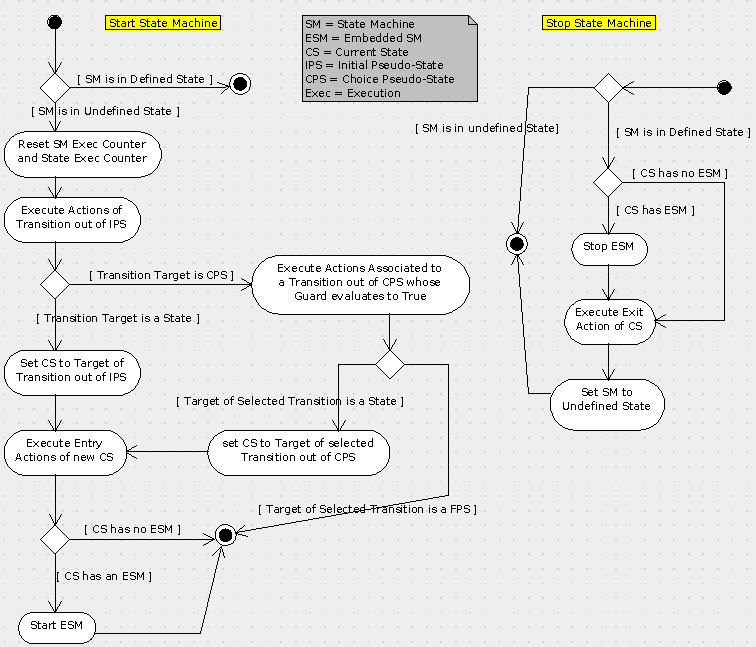
\includegraphics[scale=0.415,keepaspectratio=true]{SM_StartStop.png}
 % SMD.png: 474x227 pixel, 72dpi, 16.72x8.01 cm, bb=0 0 474 227
 \caption{Logic for the Start and Stop Commands to a State Machine}
 \label{fig:logicStartStopCmdSM}
\end{figure}

When a transition command T is sent to a state machine S, then the following behaviour is executed:

\begin{fw_enumerate}
\item If S is in an undefined state, then no further action is taken.
\item If T is the Execute command, then the execution counters of the state machine are
incremented and the do-action associated to the current state of S is
executed. If several do-actions are present, they are executed in the order in which
they are listed.
\item If S is in a defined state and the current state of S has an embedded state machine SE,
then the transition command T is propagated to SE.
\item If there are no transitions from the current state of S that have T as their trigger, then
no further action is taken.
\item If there are one or more transitions from the current state of S that have T as their
trigger, then their guards are evaluated in sequence. The order of the evaluation is
undefined. The absence of a guard is equivalent to a guard that returns TRUE.
\item When the first transition is found whose guard evaluates to TRUE, then that transition
is executed.
\end{fw_enumerate}

The logic that governs the processing of a transition command by a state machine is shown in Figure \ref{fig:logicTransitionCmdSM} as an activity diagram. 
Note that this logic merely describes the circumstances under which a transition within a state machine is executed but it does not define the logic 
according to which the transition is executed. This is done below (see also Figure \ref{fig:execTransitionSM}).

\begin{figure}[ht]
 \centering
 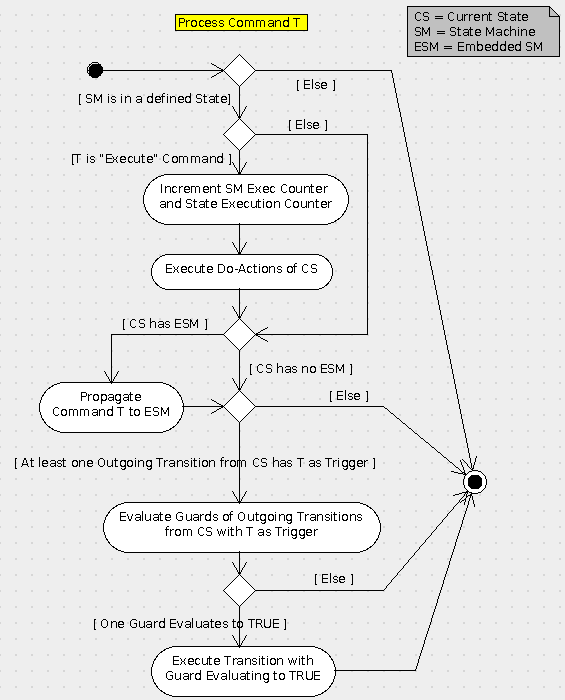
\includegraphics[scale=0.5,keepaspectratio=true]{SM_CmdProcessing.png}
 % SMD.png: 474x227 pixel, 72dpi, 16.72x8.01 cm, bb=0 0 474 227
 \caption{Logic for Processing Transition Commands by a State Machine}
 \label{fig:logicTransitionCmdSM}
\end{figure}

When a transition is executed, then the following behaviour is executed:

\begin{fw_enumerate}
\item If the source state of the transition is a state and that state has an embedded state
machine, then the embedded state machine is stopped.
\item If the source state of the transition is a state, then the exit action associated to the
source state is executed. If several exit actions are present, they are executed in the
order in which they are listed.
\item The transition action associated to the transition is executed. If several transition
actions are present, they are executed in the order in which they are listed.
\item If the target of the transition is a choice pseudo-state, then the guards of the out-going
transitions from the choice pseudo-state are evaluated in sequence until one is found
that evaluates to true and that transition is executed.
\item If the target of the transition is a final pseudo-state, then the state machine is set to an
undefined state and no further action is taken.
\item If the target state of the transition is a state, then the current state of the state machine
is updated to be equal to the target state of the transition and the state execution counter is
reset.
\item If the target state of the transition is a state, then the entry action of the target state is
executed. If several entry actions are present, they are executed in the order in which
they are listed.
\item If the target state of the transition is a state and that state has an embedded state
machine, then the embedded state machine is started.
\end{fw_enumerate}

With reference to point 4, it is noted that at least one of the guards on the outgoing transitions from a choice pseudo-state is guaranteed to be true 
because of constraint \textbf{D1} in the previous section.
The logic according to which a transition is executed is shown as an activity diagram in Figure \ref{fig:execTransitionSM}. Note that this logic is called up 
by the logic shown in the activity diagram of Figure \ref{fig:logicTransitionCmdSM}.

\begin{figure}[ht]
 \centering
 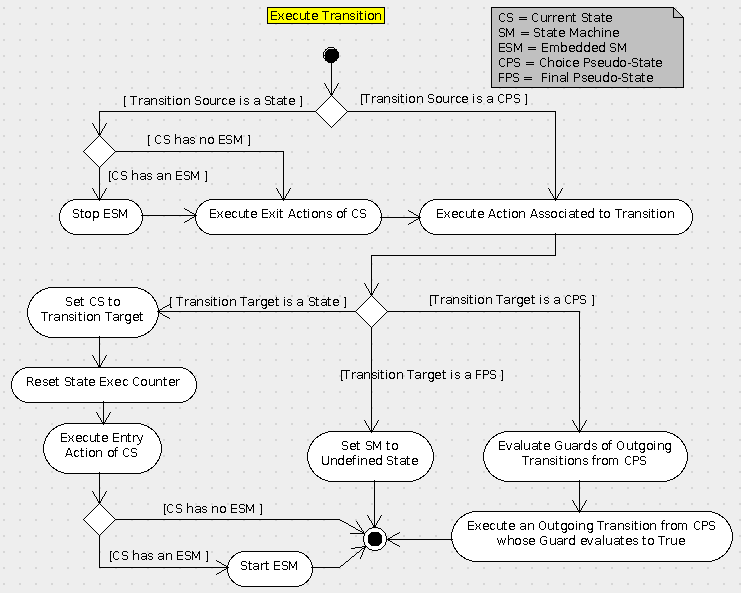
\includegraphics[scale=0.45,keepaspectratio=true]{SM_TransitionExecution.png}
 % SMD.png: 474x227 pixel, 72dpi, 16.72x8.01 cm, bb=0 0 474 227
 \caption{Logic for Executing Transitions in a State Machine}
 \label{fig:execTransitionSM}
\end{figure}

Transition commands may carry parameters. These parameters may be passed to any of the state or transition actions that are executed as part of 
the processing of the transition command.

The execution of the various actions associated to the three state machine operations is performed in sequence: an action is executed only when 
the previous one has completed. Note that, since state and transition actions are constrained to execute in zero logical execution time, 
the execution of a state machine operation will also execute in zero logical execution time.  

Transition commands arrive and are processed in sequence. A new command can only arrive and be processed by a state machine when the previous one has 
been fully processed. State machines have no queues to buffer incoming transition commands.

The above rule in particular implies that transition commands cannot be nested, namely the processing of a transition command by a state machine 
cannot result in a new command being sent to the same state machine (nesting rule).

As an example where the nesting rule would be violated, consider the following situation. A first transition command is sent to state machine A that 
triggers a transition from state A1 to state A2. The entry action of state A2 sends a second transition command to state machine A. 

As a second example of violation of the nesting rule, consider  a  transition command that is sent to state machine A that triggers a transition 
from state A1 to state A2. The entry action of state A2 sends a new transition command to state machine B. State machine B, as part of its processing 
of this command, sends a new transition command to state machine A.

Forwarding of transition commands from one state machine A to another state machine B is instead allowed provided that neither of the two state machines 
is embedded in the other one. 

Forwarding of transition commands from an embedded state machine to its embedding state machine or vice-versa is forbidden. This restriction helps 
to avoid the ambiguities that would arise when, for instance, the entry action of a state in an embedded state machine triggers a transition in 
the embedding state machine.

\subsection{UML 2 Compliance}
The state machine model offered by the FW Profile complies with the UML 2 state machine
model in the sense that the elements of the state machine concept of the FW Profile and their
semantics can be mapped in an obvious way to a subset of the elements of the state machine
concept of UML 2 with the following provisos:

\begin{fw_itemize}
\item The semantics of choice pseudo-states in the FW Profiles subsumes that of junction pseudo-states
in UML2. Thus, in the FW Profile, choice pseudo-states can also be used to join together incoming
transition flows.
\item The execution counters are specific to the FW Profile. They have been introduced as a
substitute for the concept of time (which does not exist in the FW Profile State Machines) in
the sense that, if state machines are executed periodically, then the value of their execution 
counters is proportional to the time elapsed since the state machine was started (State Machine
Execution Counter) or since the current state was entered (State Execution Counter). 
\end{fw_itemize}

It should be emphasized that the state machine model proposed by the FW Profile is far more
restrictive than that supported by UML 2. This is because the FW Profile uses state machines
to model purely functional (non-time-related) behaviour.



%===============================================================================

\section{Procedure Model of the FW Profile}\label{sec:prModel}
The C1 Implementation implements the procedure model of the FW Profile. The FW Profile is defined in reference \cite{ref:fwprofile}. For convenience, this section reports an excerpt of reference \cite{ref:fwprofile} defining the semantics of procedures.

\subsection{Definition of Procedures}
A procedure in the FW Profile consists of the following elements:

\begin{fw_itemize}
\item One \emph{initial node}
\item One or more \emph{actions nodes} (or actions)
\item One or more \emph{control flows}
\item Zero or more \emph{decision nodes}
\item Zero or more \emph{final nodes}
\item Two \emph{execution counters}
\end{fw_itemize}

The \emph{initial node} is characterized by one control flow which has the initial node as its source
and has either an action node or a decision node as its target.

An \emph{action node} (or action) is characterized by the following elements:

\begin{fw_itemize}
\item One or more incoming control flows
\item One outgoing control flow
\item The behaviour associated to the action
\end{fw_itemize}

The incoming control flows are control flows which have the action as its target. The outgoing
control flow is a control flow which has the action as its source.

An action represents a single step within a procedure. It encapsulates behaviour that is not
decomposed further within the procedure. The action's behaviour can be defined using natural
language or some formalism (e.g. an \"action language\").

A \emph{control flow} is characterized by the following elements:

\begin{fw_itemize}
\item One source
\item One target (or destination)
\item Zero or one guards
\end{fw_itemize}

The source and the target are either action nodes or decision nodes. Additionally, the initial
node can be the source of a control flow and the final node can be the destination of one or
more control flows.

The guard is a specification which evaluates either to TRUE or FALSE and which
has no side effects. Absence of a guard is equivalent to a guard which always evaluates to TRUE.

A \emph{decision node} is characterized by the following elements:
\begin{fw_itemize}
\item One or more \emph{incoming control flows}
\item Two or more \emph{outgoing control flows}
\end{fw_itemize}

The incoming control flows are control flows that have the decision node as its target. The
outgoing control flow are control flows that have the decision node as their source.

For control flows issuing from a decision node, the pre-defined \textit{Else} guard is available. This
guard returns TRUE if and only if all the other guards attached to control flows issuing from
the same decision node return FALSE.

The \emph{final node} is characterized by one or more incoming control flows (namely control flows
that have the final node as their target). Note that all final nodes are equivalent and therefore it
would be legitimate to allow only one single final node. The option to have more than one is
introduced as a matter of convenience.

The \emph{execution counters} are unsigned integers which are exclusively characterized by their value.
The first execution counter is called the \emph{Procedure Execution Counter} and the second one
is called the \emph{Node Execution Counter}.

The following syntactical constraints apply to the definition of the procedure elements:

\begin{fw_itemize}
\item C1. The control flows out of a decision node must have a guard.
\end{fw_itemize}

The following dynamical constraints must be satisfied when a procedure is executed:
\begin{fw_itemize}
\item D1. Among the outgoing control flows from a decision node, at least one must have a
guard which evaluates to true;
\item D2. The evaluation of the guards of a control flow must be free of side-effects;
\item D3. The procedure actions and guards must execute in zero logical execution time
(i.e. on an infinitely fast processor and in the absence of pre-emption or blocking, 
they must execute in zero time).
\end{fw_itemize}

The last constraint implies that the behaviour encapsulated by the actions and by the guards
must be purely functional. In practice, this means that actions and guards cannot include time-
dependent behaviour or behaviour that depends on synchronization with other flows of
executions.

The execution counters of a procedure count the number of times the procedure has
been executed (one counts the number of times the procedure has been executed since it 
was started and the other counts the number of times the procedure has been executed
since its current node was entered). Since procedures will often be executed periodically,
the execution counters can serve as proxies for measuring the elapsing of time.


\subsection{Procedure Behaviour}\label{sec:procBehaviour} 
Four operations may be performed on a procedure: (a) the procedure may be \emph{started}; (b) the
procedure may be \emph{executed}; (c) the procedure may be \emph{stopped}; or (d) the procedure may be
\emph{run}.

Procedures are purely reactive: they wait for one of these four operations to be performed upon
them and they only execute a behaviour in response to one of these operations.

Operations are performed in response to \emph{commands}: the command Start triggers the start
operation; the command Execute triggers the execute operation; the command Stop triggers the
stop operation; and the command Run triggers the run operation.

A procedure may be in two states: STOPPED or STARTED. Initially, by default, the procedure
is in state STOPPED. When the procedure is in state STARTED, it has a \emph{current node}. The
current node is either the procedure's initial node or one of its action nodes.

When a procedure is \emph{started}, the following behaviour is executed:
\begin{fw_enumerate}
\item If the procedure is in state STARTED, then no further action is performed;
\item If the procedure is in state STOPPED, then it is put in state STARTED, its current
node is set equal to its initial node and its execution counters are reset.
\end{fw_enumerate}

When a procedure is \emph{stopped}, the following behaviour is executed:

\begin{fw_enumerate}
\item If the procedure is in state STOPPED, then no further action is performed;
\item If the procedure is in state STARTED, then it is put in state STOPPED and its current
node is set to an invalid value.
\end{fw_enumerate}

Thus, the Stop and Start commands toggle the state of a procedure and update its current node.
This is shown in the state diagram of figure \ref{fig:PR_StartStop}.

\begin{figure}[ht]
 \centering
 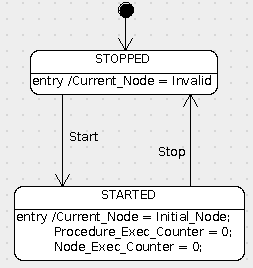
\includegraphics[scale=0.5,keepaspectratio=true]{PR_StartStop.png}
 \caption{Procedure Start/Stop Commands}
 \label{fig:PR_StartStop}
\end{figure}

When a procedure is \emph{executed}, the following behaviour is executed:
\begin{fw_enumerate}
\item If the procedure is in state STOPPED, then no further action is performed;
\item If the procedure is in state STARTED, then its execution counters are incremented
by 1 and the guard attached to the outgoing control flow of the current node is evaluated;
\item If the guard evaluates to FALSE, then no further action is performed;
\item If the guard evaluates to TRUE and the target of the outgoing control flow attached to
the current node is an action node T, then: (a) the current node is set equal to T, (b) the
node execution counter is reset, (c) the
behaviour associated to T is executed, (d) the guard on the out-going control flow of T is evaluated
and steps 3 and 4 are (recusively) repeated;
\item If the guard evaluates to TRUE and the target of the outgoing control flow attached to
the current node is a decision node, then: (a) the guards of the outgoing control flows
attached to the decision node are evaluated; (b) if the target of the outgoing control
flow whose guard evaluates to TRUE is another decision node, then steps (a) to (d) are
performed upon it; (c) if the target of the outgoing control flow whose guard evaluates
to TRUE is an action node T, then the current node is set equal to T, the behaviour
associated to T is executed, the guard on the out-going control flow of T is evaluated
and steps 3 and 4 are (recusively) repeated; (d) if the target of the
outgoing control flow whose guard evaluates to TRUE is a final node, the state of the
procedure is set to STOPPED and the current node is set equal to an invalid value.
\item If the guard evaluates to TRUE and the target of the outgoing control flow attached to
the current node is a final node, then the state of the procedure is set to STOPPED,
and the current node is set equal to an invalid value.
\end{fw_enumerate}

Thus, in summary, when a procedure is executed, it tries to traverse the control flow issuing
form the current node. If this can be done (i.e. if the guard associated to the control flow
evaluates to true), then it advances the execution of the procedure until it finds a guard that
evaluates to false or until it finds a final node. Whenever an action node is traversed, its
associated behaviour is executed.

The Execute command may carry parameters. These parameters may be passed to any of the
actions that are executed as part of the processing of the Execute command.

Note that, at any given time, only one flow of control may be traversing a procedure. This flow
of control is advanced every time that the procedure is executed.

The behaviour associated to the execution of a procedure is shown as an activity diagram in
figure \ref{fig:PR_Execution}.

Finally, when a procedure is run, the following behaviour is executed:

\begin{fw_enumerate}
\item The procedure is started;
\item The procedure is executed;
\item The procedure is stopped. 
\end{fw_enumerate}

Thus, the Run operation is defined in terms of the previous three operations. The Run
operation may take parameters which are passed to the Execute operation which is performed
as part of the Run operation (step 2 above).

The Run operation is only useful for procedures which execute in one single cycle. It is
typically used to perform the actions associated to a state in a state machine.

The execution of the various actions associated to the four procedure operations (Start,
Execute, Stop, and Run) is performed in sequence: an action is executed only when the
previous one has completed. Note that, since actions are constrained to execute in zero logical
time, the execution of a procedure operation will also execute in zero logical time.

Requests to perform an operation upon a procedure are executed in sequence. A new request
can only be processed by a procedure when the previous one has been fully processed.
Procedures have no queues to buffer incoming operation requests.

Note that the procedure operations do not return any values.

\begin{figure}[ht]
 \centering
 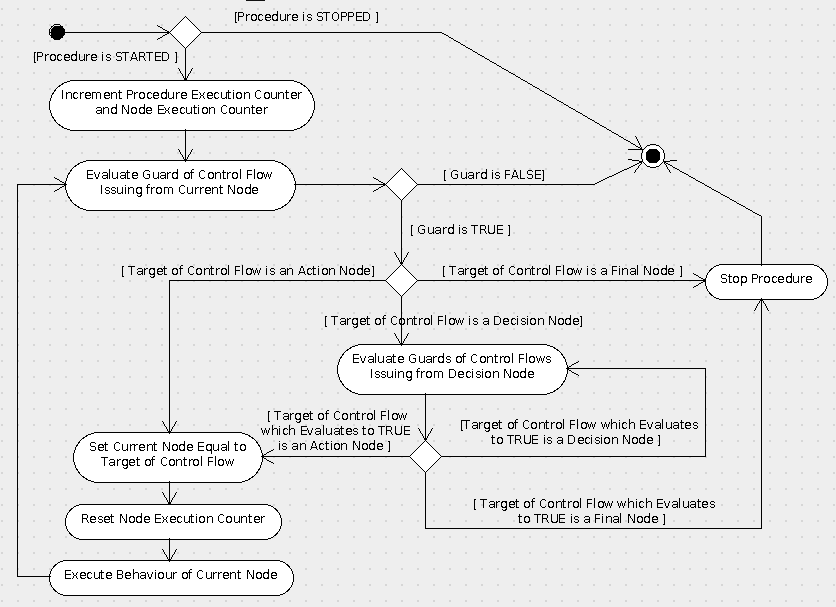
\includegraphics[scale=0.4,keepaspectratio=true]{PR_Execution.png}
 \caption{Procedure Execution Logic}
 \label{fig:PR_Execution}
\end{figure}

\subsection{UML 2 Compliance}
The procedure model offered by the FW Profile complies with the UML 2 activity model in
the sense that the elements of the procedure concept of the FW Profile and their semantics can
be mapped in an obvious way to a subset of the elements of the activity concept of UML 2.

The execution counters are specific to the FW Profile. They have been introduced as a
substitute for the concept of time (which does not exist in the FW Profile Procedures) in
the sense that, if procedures are executed periodically, then the value of their execution 
counters is proportional to the time elapsed since the procedure was started (Procedure
Execution Counter) or since the current node was entered (Node Execution Counter). 



%===============================================================================

\section{RT Container Model of the FW Profile}\label{sec:rtContainerModel}
The C1 Implementation implements the RT Container model of the FW Profile. The FW Profile is defined in reference \cite{ref:fwprofile}. For convenience, this section reports an excerpt of reference \cite{ref:fwprofile} defining the RT Container model of the FW Profile.

\subsection{Role of RT Containers}
State Machines and Procedures allow all functional aspects of a software application to be modelled. RT Containers complement them by offering a means to capture one aspect of the time-related behaviour of an application.

It is important to stress that full modelling of an application's timing behaviour is beyond the scope of the FW Profile. This is because the FW Profile is aimed at modelling individual applications. Applications normally run on a software/hardware platform which they share with other applications. Timing behaviour is a system-level aspect (it depends, for instance, on the relative priorities of the threads allocated to the various applications in a system) and cannot therefore be fully captured at application level.

RT Containers provide a way to encapsulate the activation logic for a functional behaviour. More specifically, a RT Container can be seen as a representation of a thread that controls the execution of some functional behaviour. The RT Container model defined by the FW Profile allows the conditions under which the thread is released to be specified.

Conceptually, a RT Container can be seen as a software structure that encapsulates some
functional code and endows it with certain timing properties. Thus, RT Containers are a means of separating the specification of the timing aspects of an application from its functional aspects.

There is a difference between procedures and state machines on the one hand, and RT Containers on the other hand. All three concepts are offered as means to express the behaviour of a software application but they exist at different levels of abstraction: state machines and procedures constitute a generic modelling language for the functional part of an application; RT Containers allow the timing behaviour of a software application to be modelled but they presuppose the use of certain design patterns for handling the activation of functional code. The RT Container concept is thus less generic than the state machine and procedure concepts.

The design pattern behind the concept of RT Containers is a notification-based model of thread activation where the notification can be either time-triggered or sporadic (event-driven notification).

\subsection{Definition of RT Container}
A RT Container is defined by the following elements:

\begin{itemize}[itemsep=0mm]
\item One \emph{Activation Procedure}
\item One \emph{Activation Thread}
\item One \emph{Notification Procedure} 
\end{itemize}

The \emph{Activation Procedure} is a FW Profile Procedure which executes the functional behaviour encapsulated by the RT Container.

The \emph{Activation Thread} is the thread responsible for executing the Activation Procedure (and hence for executing the functional behaviour encapsulated by the RT Container).

The \emph{Notification Procedure} is a FW Profile Procedure which encapsulates the logic for notifying the Activation Thread.

%------------------------------------------------------------------------
\subsection{RT Container Behaviour}\label{sec:rtContainersBehaviour}
Three operations may be performed on a RT Container: (a) the RT Container may be \emph{started}; (b) the RT Container may be \emph{stopped}; and (c) the RT Container may be \emph{notified}.

A RT Container may be in two states: STOPPED or STARTED. Initially, by default, the container is in state STOPPED. When a RT Container is started, the behaviour shown in the activity diagram in the left-hand side of figure \ref{fig:RTStartStop} is executed. The Start operation only has an effect if the container is in state STOPPED when the operation causes the Activation and Notification Procedures to be started and executed once and the Activation Thread to be created and released. The Notification and Activation Procedures are started "atomically" in the sense that neither procedure can be executed or stopped before both have been started. Reference to figure \ref{fig:RTContainerProcedures} shows that the first execution of the Activation and Notification Procedures results in their initialization actions being executed and, in the case of the Activation Procedure, in the first Set-Up Notification action being executed. 

\begin{figure}[ht]
 \centering
 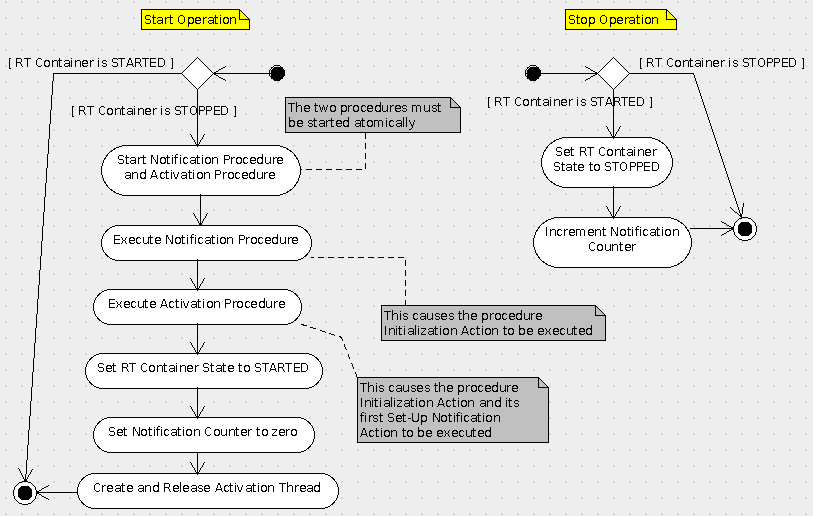
\includegraphics[scale=0.39,keepaspectratio=true]{RTStartStop.png}
 \caption{Start and Stop Operations for RT Containers}
 \label{fig:RTStartStop}
\end{figure}

When a RT Container is stopped, the behaviour shown in the activity diagram in the right-hand side of figure \ref{fig:RTStartStop} is executed. The Stop operation only has an effect if the container is in state STARTED when the operation causes the container to be placed in state STOPPED and the Notification Counter to be incremented. The latter results in one last notification being sent to the Activation Thread. This notification is necessary to ensure an orderly termination of the thread and of the Activation and Notification Procedures. 

When a RT Container is notified, the following behaviour is executed:

\begin{enumerate} 
\item If the RT Container is in state STOPPED, then no further action is performed;
\item If the RT Container is in state STARTED, then its Notification Procedure is executed.
\end{enumerate}

The behaviour of the \emph{Activation Thread} is expressed by the following pseudo-code:

\lstset{language=C,caption={Pseudo-code of Activation Thread},label=code:pseudoCodeActivationThread}
\begin{lstlisting}
while true do {
  wait until Notification Counter is greater than 0;
  decrement Notification Counter;
  execute Activation Procedure;
  
  if (Activation Procedure has terminated) then {
    put RT Container in STOPPED state;
    execute Notification Procedure;
    break;
  }

  if (RT Container is in state STOPPED) then {
    execute Activation Procedure;
    execute Notification Procedure;
    break;
  }
}
\end{lstlisting}

The thread executes a loop which starts with a check on whether there are any pending notifications (the Notification Counter holds the number of pending notifications). If there is a pending notification (i.e. if the Notification Counter is greater than zero), the thread decrements the Notification Counter and then executes the Activation Procedure (which causes the container's functional behaviour to be executed). The thread terminates when the Activation Procedure has terminated or when the RT container has been stopped. In the former case (Activation Procedure has autonomously terminated), the RT Container is put in the STOPPED state and the Notification Procedure is executed one last time before the thread exits; in the latter case (RT Container has been stopped), both procedures are executed one last time. This last execution is intended to give the procedures a chance to perform their finalization behaviour.

\begin{figure}[ht]
 \centering
 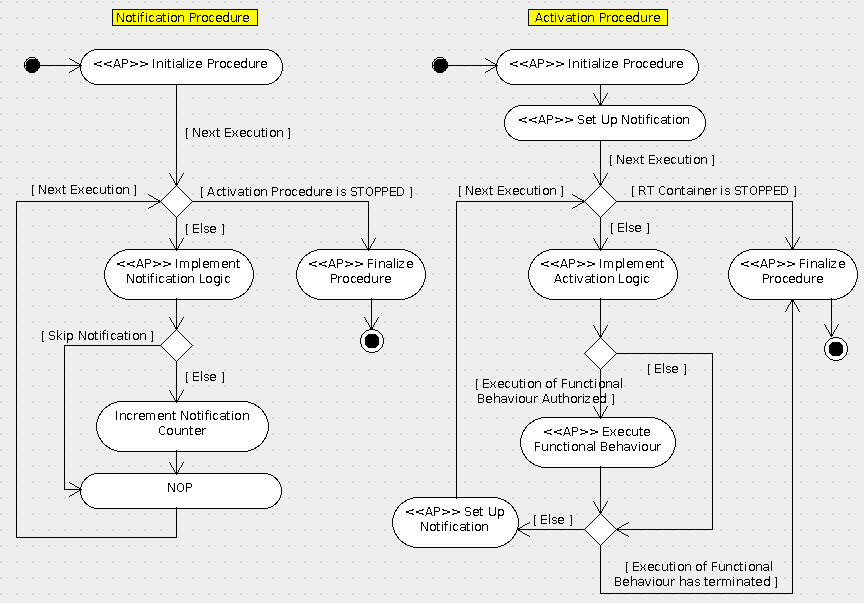
\includegraphics[scale=0.39,keepaspectratio=true]{RTContainer.png}
 % PRD.png: 474x227 pixel, 72dpi, 16.72x8.01 cm, bb=0 0 474 227
 \caption{RT Container Procedures}
 \label{fig:RTContainerProcedures}
\end{figure}

The behaviour of the \emph{Activation Procedure} and of the \emph{Notification Procedure} is shown in the
activity diagrams in Figure \ref{fig:RTContainerProcedures}. The definition of the two procedures makes use of the
“adaptation point” stereotype to identify the parts of the container behaviour which are
application-specific. Applications are therefore expected to extend the two procedures by inserting
their own application-specific behaviour (by contrast, the behaviour of the Activation Thread is invariant and is fully defined at FW Profile level).

When the Activation Procedure is executed for the first time (i.e. after the Activation Thread
has been started), it initializes itself and sets up the first notification of the Activation Thread.
The form of the notification is application-specific. Typically, the setting up of a notification
may consist of one of the following:

\begin{enumerate} 
\item A request that the Activation Thread be notified at some time in the future;
\item A call-back registration to request to be notified when a certain software condition
arises (e.g. a variable changes value, a message arrives, etc);
\item A request to be notified when a hardware interrupt is asserted.
\end{enumerate}

Note that the notification may only need to be set up once when the Activation Procedure is initialized or it may need to be set up at every execution cycle. Note also that the same RT Container may set up different notification requests in the same execution cycle or it may set up notification requests of different kinds at different execution cycles. For this reason, the "Set-Up Notification" in the Activation Procedure is placed both at the beginning of the procedure (to be executed once at initialization time) and inside the loop (to be executed after each execution of the functional behaviour).

When a notification arrives (i.e. when the user of the container executes the Notification Procedure and this increments the Notification Counter), the Activation Thread is woken up and it executes the Activation Procedure. The procedure checks whether the RT Container has been stopped. If this is the case, the procedure performs its finalization action and then terminates. Otherwise, the procedure checks whether the functional behaviour should be executed (this is done by the "Implement Activation Logic" action) and, if so, it executes it. Afterwards, the procedure sets up the next notification (if one is needed) and then checks whether the execution of the functional behaviour has been completed. If this is so, the procedure terminates. Otherwise it waits for the next notification.

The procedure initialization and finalization actions are adaptation points which are defined at application level. Similarly, the action to set up the notification for the Activation Thread and to implement the activation logic must also be defined at application level. The latter could, for instance, be used to implement a filter which decides which notifications to process and which ones to ignore.

The Notification Procedure acts as an intermediary
between the source of the notification event and the notification trigger to the Activation
Thread. Such an intermediary may be useful to: (a) filter notification events, or (b) buffer
notification requests so as to allow the Activation Procedure to handle bursts of notifications.
With reference to the activity diagram in Figure \ref{fig:RTContainerProcedures}, the filtering 
and buffering of notification requests is done in the (application-specific) action “Implement Notification Logic”.

As already noted, the Notification Procedure runs on a thread that is external to the RT
Container: the Notification Procedure is executed by an external thread when the notification
event has occurred. Thus, the logic leading to the notification of the Activation Thread is as
follows:

\begin{fw_enumerate}
\item The Activation Procedure makes a request to be notified when a certain event occurs
(this could, for instance, be done by registering with an external component to be
notified when a certain condition occurs);
\item When the event occurs, the Notification Procedure is executed by the source of the
event;
\item The Notification Procedure evaluates the event and may decide to notify the
Activation Thread;
\item The Notification Procedure notifies the Activation Thread by incrementing the Notification Counter;
\item In response to the notification, the Activation Thread executes the Activation Procedure which may execute the
functional behaviour encapsulated by the RT Container;
\item The Activation Procedure sets up the next notification request.

\end{fw_enumerate}

This cycle is broken when either the Activation Procedure decides that the execution of the
functional behaviour has been completed or when the RT Container is stopped. Either of these
events results in the RT Container and its two procedures terminating.

The Notification Procedure may be executed both by the Activation Thread and by an external thread. For this reason, in many cases, it will be necessary to ensure that it is executed in mutual exclusion.

Note finally that, in this section, the term "event" encompasses both asynchronous occurrences (such as the arrival of hardware interrupts from an external source) or synchronous occurrences (such as periodic signals generated by an operating system). 

%------------------------------------------------------------------------
\subsection{RT Container Properties and Usage Constraints}\label{sec:rtPropUsage}
The RT Container logic defined in the previous section guarantees that certain properties (the \textit{RT Container Properties}) are satisfied when the usage of the RT Container complies with certain constraints (the \textit{RT Container Usage Constraints}). The properties are listed in table \ref{tab:RTContProp} in rows P-3 to P-7. The usage constraints are listed in the same table in rows C-1 to C-3.

\begin{longtable}{|p{0.9cm}|p{10.3cm}|}
\caption{RT Container Properties and Usage Constraints} \label{tab:RTContProp}\\
\hline
\rowcolor{lightblue}
\textbf{N} & \textbf{RT Container Properties and Usage Constraint} \\
\hline\hline
\endfirsthead
\rowcolor{lightblue}
\textbf{N} & \textbf{RT Container Properties and Usage Constraint} \\
\hline\hline
\endhead
P-3 & The Activation Thread shall never deadlock. \\
\hline
P-4 & If the RT Container is stopped after the Activation Thread has been released, then, at some later time, the Activation Procedure shall terminate. \\
\hline
P-5 & If the Activation Procedure stops or terminates (it enters the STOPPED state), then,
at some later time, the RT Container shall be stopped. \\
\hline
P-6 & If the Activation Procedure stops or terminates (it enters the STOPPED state), then,
at some later time, the Notification Procedure shall terminate. \\
\hline
P-7 & Whenever the Activation Procedure is running (it is in state STARTED), then the
Notification Procedure shall be running, too (it shall be in state STARTED). \\
\hline
P-8 & If notifications cease but the RT Container and the Activation Procedure continue to run, then, at some later time, the Activation Thread shall consume all pending notifications (the Notification Counter will become equal to zero). \\
\hline
C-1 & If the RT Container is started and then, at some later time, it is stopped, then it can be re-started only after its Activation and Notification Procedures have terminated
execution and after its Activation Thread has terminated (i.e. the user of a RT Container cannot re-start it before it has completed its orderly shutdown) \\
\hline
C-2 & The Activation Procedure is started, stopped and executed exclusively by the RT
Container (i.e. the user of the container has no access to the Activation Procedure) \\
\hline
C-3 & The Notification Procedure is started and stopped exclusively by the RT Container
itself (i.e. the user of the RT Container can execute the Notification Procedure through the Notify operation but it cannot start or stop it) \\
\hline
\end{longtable}

The usage constraints define the conditions for the legal use of a RT Container. If these
constraints are satisfied, then the user can assume that the RT Container will comply with its
properties. Note that the container's properties hold under all circumstances, irrespective of the
scheduling and notification/triggering policies adopted for the Activation Thread and for the
thread controlling the Notification Procedure and irrespective of the way in which the
adaptation points in the container's procedure are filled.

Properties P-4 and P-5 guarantee that, if the RT Container is stopped or the Activation
Procedure terminates, then the entire container will terminate in the sense that the container
itself and its two procedures will all enter the STOPPED state. 
Property P-8 ensures that, if thread scheduling is fair and the rate at which notifications are generated is compatible with the rate at which they are processed, then no backlog of unprocessed notifications will build up. 

Some notifications may instead remain unprocessed if either the Activation Thread autonomously terminates or the RT Container is stopped by the user. Thus, in informal language, the semantics of the Stop operation on the RT Container is not: "Process all pending notifications and then terminate"; but rather: "Discard any pending notifications and then terminate". 

Note that the container's procedures can only terminate execution “naturally” (as opposed to
being forcefully stopped). This is because the RT Container logic never stops them and usage
constraints C-2 and C-3 ensure that they are not stopped by any external agent. This is
important because it means that the procedure will always execute their finalization behaviour
before terminating.

Constraint C-1 states that a RT Container can only be re-started after it has completed its
shutdown. This is a legitimate constraint because properties P-4 and P-6 guarantee that,
if the container is stopped, then its two procedures will eventually terminate. This means that
the user of a RT Container can always rely on the container completing its shutdown in a finite
amount of time.



\newpage

\begin{thebibliography}{6}
 
\bibitem{ref:fwprofile} Alessandro Pasetti, Vaclav Cechticky:
           {\sl The FW Profile}. PP-DF-COR-00001, Revision 1.3.0,
           P\&P Software GmbH, Switzerland, 2013 

\bibitem{ref:reqs} Alessandro Pasetti, Vaclav Cechticky:
           {\sl The Framework Profile - C1 Implementation User Requirements}. 
           PP-SP-COR-00001, Revision 1.2.0,
           P\&P Software GmbH, Switzerland, 2013 

\end{thebibliography}

\end{document}          

